\chapter[Pointer Swizzling in the DBMS Buffer Management]{Pointer Swizzling as in ``In-Memory Performance for Big Data'' \cite{Graefe:2014}} \label{ch:paper}

\section[Definition of a Database Management System]{Definition of a Database Management System}

    A \emph{database} is a collection of persistently stored data that should be somehow used by application programs. Mainly to reduce the complexity of application programs (especially of information systems) that access such databases, a specialized kind of software evolved in the mid-1960's that takes care about the database access - the \emph{database management system} (\emph{DBMS}). Early works on database management systems were e.g. done in the \emph{Data Base Task Group} of the \emph{CODASYL} which was founded in 1965 \cite{wikipedia.En_Data_Base_Task_Group}. To fulfil this task, according to \cite{GarciaMolina:2009} a DBMS is expected to offer the following features:
    \begin{itemize}
        \item Offer an interface to \emph{create new databases} and to define the \emph{logical structure of the data}.
        \item Offer an interface to \emph{query} and \emph{modify} the data.
        \item \emph{Persistently} store \emph{very large amounts of data} that can be accessed with a \emph{high performance}.
        \item Offer \emph{ACID} \cite{HaerderReuter83} properties.
    \end{itemize}

\section[Structure of a DBMS]{The Structure of a Database Management System}

    Just like any other complex software system (as well as other complex systems), a database management system can't be designed and implemented monolithic but it needs to be well-structured to reduce its complexity as ``systematic abstraction is the prime task of computer science'' (\emph{H. Wedekind}). A typical structure of a DBMS is based on a layer architecture which defines a number of layers, where each layer only has interfaces to the over- and underlying layer.

\subsection[ANSI/SPARC DBMS Model]{The ANSI/SPARC DBMS Model}

    The \emph{ANSI/SPARC DBMS Model} \cite{Jardine:1976} offers a conceptual, three-layer architecture that divides a data independent DBMS as seen in figure \ref{fig:ansisparcarchitecture}. The model defines finer-grained architectures as well but the understanding of those isn't needed for the classification of the buffer management as component of a DBMS.

\begin{@empty}
    \tikzset{%
        every node/.style = {font = \sffamily},
        application/.style = {rectangle, draw, thick},
        layer/.style = {rectangle, draw, thick},
        external/.style = {layer},
        conceptual/.style = {layer},
        internal/.style = {layer},
        disk/.style = {cylinder, cylinder uses custom fill, shape border rotate = 90, draw, minimum height = 1cm, minimum width = 1.5cm, thick},
        interfacearrow/.style = {<->, thick, draw = black}
    }

    \nottoggle{bwmode}{
        \tikzset{%
            application/.append style = {color = Black, fill = Black!15},
            external/.append style = {color = OliveGreen, fill = OliveGreen!15},
            conceptual/.append style = {YellowOrange, fill = YellowOrange!15},
            internal/.append style = {color = Red, fill = Red!15},
            disk/.append style = {color = Blue, cylinder body fill = Blue!15, cylinder end fill = Blue!40}
        }
    }

    \begin{figure}[ht!]
        \centering
        \scalebox{1}{
            \begin{tikzpicture}[node distance = 4ex]
                \node[application]								(app2) 	[]				{\begin{tabular}{c}Application\\Program\end{tabular}};
				\node[application]								(app1) 	[left = of app2]		{\begin{tabular}{c}Application\\Program\end{tabular}};
				\node[application]								(app3) 	[right = of app2]		{\begin{tabular}{c}Application\\Program\end{tabular}};
				\node[draw = none]								(extlay)	[below = of app2]	{};
				\node[external]									(ext1)	[left = of extlay]		{External Level};
				\node[external]									(ext2)	[right = of extlay]	{External Level};
				\node[conceptual]								(con)		[below = of extlay]	{Conceptual Level};
				\node[internal]									(int)		[below = of con]	{Internal Level};
				\node[disk]									(dis2) 	[below = of int]		{};
				\node[disk]									(dis1) 	[left = of dis2]		{};
				\node[disk]									(dis3) 	[right = of dis2]		{};
				
				\path[interfacearrow]		(app1)		--		(ext1);
				\path[interfacearrow]		(app2)		--		(ext1);
				\path[interfacearrow]		(app3)		--		(ext2);
				\path[interfacearrow]		(ext1)		--		(con);
				\path[interfacearrow]		(ext2)		--		(con);
				\path[interfacearrow]		(con)			--		(int);
				\path[interfacearrow]		(int)			--		(dis1);
				\path[interfacearrow]		(int)			--		(dis2);
				\path[interfacearrow]		(int)			--		(dis3);
			\end{tikzpicture}
		}
        \vspace{.75em}
		\caption{ANSI-SPARC Architecture for Databases}
		\label{fig:ansisparcarchitecture}
	\end{figure}
\end{@empty}

    The \emph{abstraction} of the data representation increases from the lowermost to the uppermost layer in this model. The \emph{application programs} access the \emph{user representations} of the database provided by the \emph{external layers}. This representation offers different views on the database depending on the \emph{specific application program needs}. The \emph{conceptual level} offers a \emph{holistic representation} of the data which corresponds to the \emph{data model} of the DBMS that can be e.g. relational or object-oriented. The \emph{internal layer} stores a \emph{physical representation} of the data on the \emph{disk(s)} \cite{udemy_ANSI-SPARC}. The main concern of these layers is to offer \emph{physical} (internal layer), \emph{logical} (conceptual layer) and \emph{data independence} and \emph{distribution independence} (internal layer).

\subsection[5-Layer DBMS Architecture]{The 5-Layer DBMS Architecture}

    The implementation of a DBMS can't be based directly on this conceptual model because it only defines some levels to achieve data independence. It can only be used for a very coarse-grained assignment of functionality to the different layers. Therefore there are many other architectures roughly based on the \emph{ANSI/SPARC DBMS Model} that enable a systematical implementation of a DBMS. One of those is the five-layer architecture \cite{Haerder:1983} \cite{Haerder:1985} that assigns concrete functionality to its layers and that defines the interfaces between these layers as in figure \ref{fig:fivelayerarchitecture}. The following description will be top-down as the buffer management can be found in the lower part of the architecture.

\begin{@empty}
    \tikzset{%
        every node/.style = {font = \sffamily},
        layer/.style = {rectangle, draw, thick},
        application/.style = {layer},
        datastructures/.style = {layer},
        accesspaths/.style = {layer},
        storagestructures/.style = {layer},
        propagationcontrol/.style = {layer},
        fileservices/.style = {layer},
        disk/.style = {cylinder, cylinder uses custom fill, shape border rotate = 90, draw, minimum height = 1cm, minimum width = 4cm, thick},
        disktext/.style = {},
        interfacearrow/.style = {<->, thick, draw = black}
    }

    \nottoggle{bwmode}{
        \tikzset{%
            application/.append style = {color = Black, fill = Black!15},
            datastructures/.append style = {color = YellowOrange, fill = YellowOrange!15},
            accesspaths/.append style = {color = RedOrange, fill = RedOrange!15},
            storagestructures/.append style = {color = Red, fill = Red!15},
            propagationcontrol/.append style = {color = BrickRed, fill = BrickRed!15},
            fileservices/.append style = {color = Purple, fill = Purple!15},
            disk/.append style = {color = Blue, cylinder body fill = Blue!15, cylinder end fill = Blue!40},
            disktext/.append style = {color = Blue},
        }
    }

    \begin{figure}[ht!]
        \centering
        \scalebox{1}{
            \begin{tikzpicture}[node distance = 5ex]
                \node[application]							(tp)			[]				{Transaction Programs};
				\node[datastructures]						(lgs)			[below = of tp]		{Logical Data Structures};
				\node[accesspaths]							(lap)			[below = of lgs]		{Logical Access Paths};
				\node[storagestructures]						(ss)			[below = of lap]		{Storage Structures};
				\node[propagationcontrol]						(pc)			[below = of ss]		{Propagation Control};
				\node[fileservices]							(fs)			[below = of pc]		{File Services\vphantom{g}};
					
				\node[disk]								(storage)		[below = of fs]		{};
		
				\node at (storage)	[disktext]					(storaget)		[]				{\small Secondary Storage};

				\path[interfacearrow]		(tp)		--	node[left]	{Set-Oriented Interface}		node[right]	{\emph{SQL, QBE}}													(lgs);
				\path[interfacearrow]		(lgs)		--	node[left]	{Record-Oriented Interface}	node[right]	{\small \lstinline|next()|\emph{, }\lstinline|remove()|\emph{, }\lstinline|add()| record}	(lap);
				\path[interfacearrow]		(lap)		--	node[left]	{Internal Record Interface}		node[right]	{\emph{store record in index}}											(ss);
				\path[interfacearrow]		(ss)		--	node[left]	{Buffer Interface}			node[right]	{\small \lstinline|fix()|\emph{, }\lstinline|unfix()|\emph{, }\lstinline|refix()|\emph{ page}}	(pc);
				\path[interfacearrow]		(pc)		--	node[left]	{File Interface}				node[right]	{\small \lstinline|fread()|\emph{, }\lstinline|fwrite()|\emph{ block}}					(fs);
				\path[interfacearrow]		(fs)		--	node[left]	{Device Interface}			node[right]	{\emph{channel programs}}											(storage);
            \end{tikzpicture}
        }
        \vspace{.75em}
        \caption{Five Layer Architecture for DBMS}
        \label{fig:fivelayerarchitecture}
    \end{figure}
\end{@empty}

    The \emph{transaction programs} use the \emph{set-oriented interface} of the layer of \emph{logical data structures} (\emph{non-procedural access layer}). This interface is usually very powerful and offers the capabilities to process complex descriptive DBMS query languages like \emph{SQL}, \emph{QBE} or \emph{XQuery} as input. As the identifiers used by these languages are part of the metadata, this layer is responsible to map those to the internal identifiers of the \emph{record-oriented interface}. Like all the other components of a DBMS, this layer uses the \emph{metadata management system} to store its metadata which are e.g. metadata that describe structures like \emph{relations}, \emph{views} and \emph{tuples}. This layer also needs to map the complex set operators of the \emph{set-oriented interface} to those simple ones of the \emph{record-oriented interface}, that usually uses an \emph{iterator}-like interface on records. The \emph{non-procedural access layer} also has to offer data integrity, access control, transaction management and it is the most import layer for the \emph{query optimizer}.

    The \emph{navigational access layer} which operates on \emph{logical access paths} uses the \emph{internal record interface} to offer navigational access though the records to the overlying layer. The control over the returned records is very limited at this interface. E.g. a selection (based on explicit attribute values) of records from a specific set can be returned one-record-at-a-time where the overlying layer can iterate over. The layer needs to process the sorting and it has to navigate through the access path structures provided by the \emph{internal record interface}. The internal records, provided by the underlying layer are also of a different format (e.g. datatypes) as the external records are and therefore a mapping is required here. The \emph{record-oriented interface} would be the uppermost interface of navigational or hierarchical DBMS.

    The \emph{record and access path management} offers access to \emph{access path structures} like B* trees or hash indexes through the \emph{internal record interface}. This layer has to manage the mapping between records and pages as the interface below only offers pages whereas the \emph{internal record interface} uses records as addressing unit. The importance to realize such \emph{index structures} in a separate layer is quite high compared to the layers above because the selection of the best fitting \emph{index structure} is mandatory for the performance of the whole DBMS and the later extension in this area is quite probable. For one-dimensional data, this probably doesn't hold as B* tree and hash indexes usually offer high performance (regarding to metrics like storage overhead, insert, update, delete and search performance) for that case. But there isn't a single multi-dimensional index structure that always nearly outperforms all the other ones. A comprehensive but far not complete and especially not very recent (there is still a lot of research done in that field) overview of such multi-dimensional access paths can be found in \cite{Gaede:1998}. Many implementations of general purpose DBMS offer multiple \emph{index structures} and secondary indexes which are both features that needs to be supported by this layer. There are also multiple addressing schemes available, to locate records inside pages which is important for the \emph{index structures} and other features of this layer. Other common capabilities of the \emph{record and access path management} are support for variable-sized fields, large fields that are stored out-of-line and references between records.

    The \emph{propagation control} offers the \emph{buffer interface} with pages as addressing units. As the overlying layers only process data in main memory and as the \emph{file services} only offer file streams, this layer is used to provide an image of the persistently stored data in memory. 

    The \emph{file management} offers \emph{file services} through the \emph{file interface}. It needs to abstract from the \emph{device interface} offered by the \emph{secondary storage devices} to offer dynamically growing files and blocks of different length within those files to the overlying layer. Therefore it needs to manage data structures to store file addresses (on the storage device) and block borders as well as addresses of unused parts of the \emph{secondary storage devices}. It needs to take into account the special characteristics of the used storage device like HDDs and SSDs. Especially HDDs with its physical addressing based on cylinders, tracks and sectors aren't trivial to abstract from. Consecutive blocks within a file should be e.g. located on cylinders that are physically close together to decrease the access latency by reducing the number of random accesses.

    A more detailed discussion of the design and implementation of a DBMS is beyond the scope of this work. Comprehensive descriptions on this topic can be found in \cite{GarciaMolina:2009}, \cite{Datenbanksysteme_-_Konzepte_und_Techniken_der_Implementierung} and \cite{Datenbanken_-_Implementierungstechniken}.

\subsection[Motivation for a DBMS Buffer]{Motivation for the Usage of a DBMS Buffer} \label{subsec:motivationbuffer}

    Just like any other software system that needs non-volatile storage with high capacity or network access, a DBMS suffers from high \emph{I/O latency}. The \emph{non-volatility} is needed to guarantee the durability of the database and the support for \emph{high capacity} is a requirement as many OLTP databases are quite large in size. 

\begin{@empty}
    \tikzset{%
        changes/.style = { -> , very thick, > = stealth}
    }
    
    \nottoggle{bwmode}{
        \tikzset{%
            volatile/.style = {fill = red!50},
            nonvolatile/.style = {fill = green!50},
            changes/.append style = {color = red}
        }
    }{
        \tikzset{%
            volatile/.style = {pattern = crosshatch, pattern color = black!25},
            nonvolatile/.style = {pattern = crosshatch dots, pattern color = black!25}
        }
    }

    \begin{figure}
    \centering
    \begin{minipage}{\linewidth}
        \resizebox{\textwidth}{!}{%
            \begin{tikzpicture}[font = \sffamily]
                % Center points of the baseline of each pyramid layer (0: Peak of the pyramid; 1: Center of the baseline of the top layer; ...)
                \node[]  (0)                                                                       {};
                \node[]  (1)   [below = 1.5cm of 0.center, anchor = center]                        {};
                \node[]  (2a)  [below = (1/3)*1.25cm of 1.center, anchor = center]                 {};
                \node[]  (2b)  [below = (1/3)*1.25cm of 2a.center, anchor = center]                {};
                \node[]  (2c)  [below = (1/3)*1.25cm of 2b.center, anchor = center]                {};
                \node[]  (3)   [below = 0.75cm of 2c.center, anchor = center]                      {};
                \node[]  (4)   [below = 0.75cm of 3.center, anchor = center]                       {};
                \node[]  (5)   [below = 0.75cm of 4.center, anchor = center]                       {};
                \node[]  (6)   [below = 0.75cm of 5.center, anchor = center]                       {};

                % Anchor points of the pyramid (n0: Left anchor point; n1: Right anchor point):
                \node[]  (10)  [left = (2/3)*1.5cm of 1.center, anchor = center]                   {};
                \node[]  (11)  [right = (2/3)*1.5cm of 1.center, anchor = center]                  {};
                \node[]  (2a0) [left = (2/3)*(1.5cm+(1/3)*1.25cm) of 2a.center, anchor = center]   {};
                \node[]  (2a1) [right = (2/3)*(1.5cm+(1/3)*1.25cm) of 2a.center, anchor = center]  {};
                \node[]  (2b0) [left = (2/3)*(1.5cm+(2/3)*1.25cm) of 2b.center, anchor = center]   {};
                \node[]  (2b1) [right = (2/3)*(1.5cm+(2/3)*1.25cm) of 2b.center, anchor = center]  {};
                \node[]  (2c0) [left = (2/3)*(1.5cm+(3/3)*1.25cm) of 2c.center, anchor = center]   {};
                \node[]  (2c1) [right = (2/3)*(1.5cm+(3/3)*1.25cm) of 2c.center, anchor = center]  {};
                \node[]  (30)  [left = (2/3)*3.5cm of 3.center, anchor = center]                   {};
                \node[]  (31)  [right = (2/3)*3.5cm of 3.center, anchor = center]                  {};
                \node[]  (40)  [left = (2/3)*4.25cm of 4.center, anchor = center]                  {};
                \node[]  (41)  [right = (2/3)*4.25cm of 4.center, anchor = center]                 {};
                \node[]  (50)  [left = (2/3)*5cm of 5.center, anchor = center]                     {};
                \node[]  (51)  [right = (2/3)*5cm of 5.center, anchor = center]                    {};
                \node[]  (60)  [left = (2/3)*5.75cm of 6.center, anchor = center]                  {};
                \node[]  (61)  [right = (2/3)*5.75cm of 6.center, anchor = center]                 {};

                % "Center" of the pyramid (shifted towards top) used for the designation of performance measures:
                \node[]  (cen) [below = 2.5cm of 0.center]                                         {};

                % Designation of performance measures:
                \node[rotate = 55]  (cpu) [left = 3.5cm of cen.center, anchor = center]  {\footnotesize \textit{\textbf{Capacity per CPU}}};
                \node[rotate = -55] (acc) [right = 4.5cm of cen.center, anchor = center] {\footnotesize \textit{\textbf{Access time}}};

                % Fills the pyramid to mark volatile and non-volatile layers:
                \fill[volatile]    (0.center) -- (30.center) -- (31.center) -- cycle;
                \fill[nonvolatile] (30.center) -- (31.center) -- (61.center) -- (60.center) -- cycle;

                % Key the markings for volatile and non-volatile layers
                \node[draw, volatile]    (red)      [left = 4cm of 0.center, anchor = north]      {};
                \node[]                  (legred)   [right = 0cm of red.east, anchor = west]      {\footnotesize Volatile};
                \node[draw, nonvolatile] (green)    [below = 0.2cm of red.south, anchor = north]  {};
                \node[]                  (leggreen) [right = 0cm of green.east, anchor = west]    {\footnotesize Non-volatile};

                % Storage layer names:
                \node[] (reg) [above = 0cm of 1.center, anchor = south]     {\footnotesize Registers};
                \node[] (l1)  [above = 0cm of 2a.center, anchor = south]    {\footnotesize L1 cache};
                \node[] (l2)  [above = 0cm of 2b.center, anchor = south]    {\footnotesize L2 cache};
                \node[] (l3)  [above = 0cm of 2c.center, anchor = south]    {\footnotesize L3 cache};
                \node[] (mem) [above = 0.05cm of 3.center, anchor = south]  {\small Main memory};
                \node[] (ssd) [above = 0.05cm of 4.center, anchor = south]  {\small Online storage \scriptsize \textit{(secondary s.) - SDD}};
                \node[] (mas) [above = 0.05cm of 5.center, anchor = south]  {\small Online storage \scriptsize \textit{(secondary s.) - HDD}};
                \node[] (mem) [above = 0.05cm of 6.center, anchor = south]  {\small Offline storage \scriptsize \textit{(tertiary storage)}};

                % Anchor points for the brace used to mark the example data from Intel Xeon:
                \node[] (0h)        [right = 2.75cm of 0]     {};
                \node[] (31h)       [right = 2.75cm of 31]    {};

                % Draw the pyramid:
                \path[ - , thick]
                (0.center)         edge        (10.center)
                (0.center)         edge        (11.center)
                (10.center)        edge        (11.center)
                (10.center)        edge        (2a0.center)
                (11.center)        edge        (2a1.center)
                (2a0.center)       edge        (2a1.center)
                (2a0.center)       edge        (2b0.center)
                (2a1.center)       edge        (2b1.center)
                (2b0.center)       edge        (2b1.center)
                (2b0.center)       edge        (2c0.center)
                (2b1.center)       edge        (2c1.center)
                (2c0.center)       edge        (2c1.center)
                (2c0.center)       edge        (30.center)
                (2c1.center)       edge        (31.center)
                (30.center)        edge        (31.center)
                (30.center)        edge        (40.center)
                (31.center)        edge        (41.center)
                (40.center)        edge        (41.center)
                (40.center)        edge        (50.center)
                (41.center)        edge        (51.center)
                (50.center)        edge        (51.center)
                (50.center)        edge        (60.center)
                (51.center)        edge        (61.center)
                (60.center)        edge        (61.center);

                % Draw the connections between the brace used to mark the example data from Intel Xeon and the appropriate pyramid layers:
                \path[dotted]
                (0.center)             edge        (0h.center)
                (31.center)            edge        (31h.center);

                % Add the capacities:
                \draw [decorate, decoration = {brace, mirror, amplitude = 3.75pt}]
                (0.center) -- (10.center) node[black, midway, xshift = -0.1cm, yshift = 0.1cm, anchor = east] {\SI{128}{\byte}\protect\footnote{Only general purpose registers are considered}};
                \draw [decorate, decoration = {brace, mirror, amplitude = 3.75pt}]
                (10.center) -- (2a0.center) node[black, midway, xshift = -0.1cm, yshift = 0.1cm, anchor = east] {\small \SI{256}{\kibi\byte}};
                \draw [decorate, decoration = {brace, mirror, amplitude = 3.75pt}]
                (2a0.center) -- (2b0.center) node[black, midway, xshift = -0.1cm, yshift = 0.1cm, anchor = east] {\small \SI{1}{\mebi\byte}};
                \draw [decorate, decoration = {brace, mirror, amplitude = 3.75pt}]
                (2b0.center) -- (2c0.center) node[black, midway, xshift = -0.1cm, yshift = 0.1cm, anchor = east] {\small \SI{8}{\mebi\byte}};
                \draw [decorate, decoration = {brace, mirror, amplitude = 3.75pt}]
                (2c0.center) -- (30.center) node[black, midway, xshift = -0.1cm, yshift = 0.1cm, anchor = east] {\SI{64}{\gibi\byte}};
                \draw [decorate, decoration = {brace, mirror, amplitude = 3.75pt}]
                (30.center) -- (40.center) node[black, midway, xshift = -0.1cm, yshift = 0.1cm, anchor = east] {\si{\tebi\byte}};
                \draw [decorate, decoration = {brace, mirror, amplitude = 3.75pt}]
                (40.center) -- (50.center) node[black, midway, xshift = -0.1cm, yshift = 0.1cm, anchor = east] {\si{\tebi\byte}--\si{\pebi\byte}};
                \draw [decorate, decoration = {brace, mirror, amplitude = 3.75pt}]
                (50.center) -- (60.center) node[black, midway, xshift = -0.1cm, yshift = 0.1cm, anchor = east] {\si{\pebi\byte}};

                % Add the access times:
                \draw [decorate, decoration = {brace, amplitude = 3.75pt}]
                (0.center) -- (11.center) node[black, midway, xshift = 0.1cm, yshift = 0.1cm, anchor = west] {\SI{1}{\cy} $\approx$ \SI{0.25}{\nano\second}};
                \draw [decorate, decoration = {brace, amplitude = 3.75pt}]
                (11.center) -- (2a1.center) node[black, midway, xshift = 0.1cm, yshift = 0.1cm, anchor = west] {\small \SI{4}{\cy} $\approx$ \SI{1}{\nano\second}};
                \draw [decorate, decoration = {brace, amplitude = 3.75pt}]
                (2a1.center) -- (2b1.center) node[black, midway, xshift = 0.1cm, yshift = 0.1cm, anchor = west] {\small \SI{12}{\cy} $\approx$ \SI{3}{\nano\second}};
                \draw [decorate, decoration = {brace, amplitude = 3.75pt}]
                (2b1.center) -- (2c1.center) node[black, midway, xshift = 0.1cm, yshift = 0.1cm, anchor = west] {\small \SI{42}{\cy} $\approx$ \SI{11}{\nano\second}};
                \draw [decorate, decoration = {brace, amplitude = 3.75pt}]
                (2c1.center) -- (31.center) node[black, midway, xshift = 0.1cm, yshift = 0.1cm, anchor = west] {\SI{51}{\nano\second}};
                \draw [decorate, decoration = {brace, amplitude = 3.75pt}]
                (31.center) -- (41.center) node[black, midway, xshift = 0.1cm, yshift = 0.1cm, anchor = west] {$\approx$ \SI{0.1}{\milli\second} \tiny \footnote{\url{http://www.samsung.com/global/business/semiconductor/minisite/SSD/M2M/download/01_Why_SSDs_Are_Awesome.pdf}}};
                \draw [decorate, decoration = {brace, amplitude = 3.75pt}]
                (41.center) -- (51.center) node[black, midway, xshift = 0.1cm, yshift = 0.1cm, anchor = west] {\numrange{5}{20}\si{\milli\second} \tiny \footnote{\url{http://www.tomshardware.de/enterprise-hdd-sshd,testberichte-241390-6.html}} \footnote{\url{https://www.computerbase.de/2016-08/seagate-enterprise-capacity-3.5-hdd-10tb-test/3/\#diagramm-zugriffszeiten-lesen-h2benchw-316}}};
                \draw [decorate, decoration = {brace, amplitude = 3.75pt}]
                (51.center) -- (61.center) node[black, midway, xshift = 0.1cm, yshift = 0.1cm, anchor = west] {$s - min$};

                % Mark the source of the performance data of the volatile layers:
                \draw [decorate, decoration = {brace, amplitude = 3.75pt}]
                (0h.center) -- (31h.center) node[black, midway, xshift = -0.625cm, yshift = 0.1cm, anchor = west] {\footnotesize \begin{tabular}{r}\textit{\textbf{Example system:}}\\\textit{Intel\textsuperscript{\tiny\textregistered} Xeon\textsuperscript{\tiny\textregistered}}\\\textit{E3-1280 v5}\\\textit{(Skylake)}\footnote{\url{https://www.7-cpu.com/cpu/Skylake.html}}\end{tabular}};

                % Orientation of changes of performance data:
                \path[changes]
                ([xshift = (-1/3)*4cm+0.25cm]60.center) edge node[above, rotate = 90]  {\footnotesize Price per capacity} ([xshift = (-1/3)*14cm-0.25cm]0.center)
                ([xshift = (1/3)*18cm+0.5cm]0.center)   edge node[above, rotate = -90] {\footnotesize Access time}        ([xshift = (1/3)*8cm]61.center);
            \end{tikzpicture}
        }
        \end{minipage}
    \vspace{.5em}
    \caption[Storage hierarchy of computer systems]{Storage hierarchy of computer systems}
    \label{fig:storagehierarchy}
    \protect
    \end{figure}
\end{@empty}

    The seriousness of the problem of \emph{I/O latency} can be seen in the storage hierarchy of a modern computer shown in figure \ref{fig:storagehierarchy}. The \emph{access time gap} between main memory and traditional HDDs is \emph{more than 6 orders of magnitude} (still 5 orders of magnitude for SSDs) in size and in addition an I/O access requires a call to the OS which needs $\approx$\numrange{2000}{5000} instructions compared to $\approx$\num{100} instructions needed for a memory access. This makes access to online storage much more expensive than main memory access and therefore a system that frequently needs to access data (in worst-case random accesses are needed), wouldn't be able to achieve an adequate performance.

\begin{@empty}
    \begin{table}[h]
        \centering
        \begin{minipage}{\linewidth}
            \footnotesize
            \begin{tabular}{|m{.15\textwidth}|m{.09\textwidth}|m{.11\textwidth}|m{.09\textwidth}|m{.09\textwidth}|m{.09\textwidth}|m{.09\textwidth}|}
				\hline
				\textbf{Hierarchy Layer} 							& \multicolumn{2}{c|}{\textbf{Main Memory}}							& \multicolumn{4}{c|}{\textbf{Secondary Storage}}	\\ \hline
				\textbf{Device Type}     							& \centering DDR4-SDRAM		& \centering DDR4-SDRAM with ECC		& \centering HDD																													& \centering Server HDD\footnote{Suitable for Server and Datacenter}		& \centering SSD					& \centering Server SSD\footnote{Interface: SAS, PCIe or FC}	\\ \hline
				\textbf{Price $\left[\si{\euro\per\giga\byte}\right]$}    	& \multicolumn{1}{r|}{\num{>5.4}}	& \multicolumn{1}{r|}{\num{>5.8}}		& \multicolumn{1}{r|}{\num{>0.027}}																								& \multicolumn{1}{r|}{\num{>0.24}}						& \multicolumn{1}{r|}{\num{>0.23}}	& \multicolumn{1}{r|}{\num{>0.35}}	\\ \hline
            \end{tabular}
        \end{minipage}
        \caption[Price per Capacity of Different Types of Memory/Storage]{Price per Capacity of Different Types of Memory/Storage Devices \textit{(as of Feb. 8, 2017)} \footnote{\url{https://www.heise.de/preisvergleich/?m=1}}} \label{tab:memorystorageprices}
    \end{table}
\end{@empty}

    Therefore it would be better to just store the database in main memory. A very crucial problem of this solution would be the \emph{available capacity} of main memory which is much smaller than the capacity of secondary memory devices. One reason for that is the much higher price of main memory as shown in table \ref{tab:memorystorageprices}. The same capacity of main memory costs more than 20-times the money than non-volatile storage devices with high performance and even 200-times the money than slow HDDs. It's also possible to connect much more secondary storage devices to one CPU as the performance of the needed bus interface of main memory doesn't allow a distance of more than a few centimeters. The higher number of CPUs (and the high price of those) needed for the same capacity of main memory makes it evermore reasonable to use secondary storage when high storage capacity is needed. As long as the needed performance doesn't really requires to have the whole database in main memory, it's impractical to store it only there.

    Also because of the need for \emph{durability} in a DBMS with ACID properties, \emph{non-volatile} storage devices to store the database on are required. In case of a crash, a database stored in main memory would be lost and therefore the effect of every committed transaction needs to be stored on a secondary storage device.

    But it's also important to make the data available on a \emph{byte-wise addressable device} as the CPU can't process data directly on \emph{block-wise addressable devices} like SSDs and HDDs. The architecture of typical computer systems requires the main memory as an intermediate link between I/O devices and the CPU (using DMA to perform well \cite{Stallings:2013}) and therefore the usage of main memory is necessary.

    Summarizing the arguments from before, it's necessary for a DBMS to \emph{use the whole storage hierarchy}. The registers are taken into account by the compiler used to compile the DBMS as well as used to compile queries generated by the query optimizer. The CPU caches are managed by cache controllers of the CPU and therefore the DBMS doesn't need to take care about the usage of those caches. But to optimize the memory usage to fit to specific characteristics of the cache controller might be promising. Some DBMS use tertiary storage to store archive and backup data on it. As those data isn't randomly accessed, the long access time of magnetic tapes (in tape libraries) doesn't matter. The long lifetime, high capacity and low price (a magnetic tape can just be stored in a shelf and doesn't require a connection to a computer) of those storage media makes it appropriate for that purpose.

    The usage of main memory as \emph{cache} for data stored on secondary storage, would therefore be the obvious solution for those remaining two layers of the storage hierarchy, as this mechanism is typically used in situations where one layer of the storage hierarchy doesn't fit the needs. The caching could be left to the operating system and its \emph{virtual memory management}. This would e.g. allow the mapping of files, stored on a block device, to main memory using \lstinline{mmap}. While this function fits the needs of the database, some properties of it makes the usage of those services for the given purpose impossible. The OS services would allow the access of persistently stored files through main memory managed with hardware acceleration. But the interface of those services isn't sufficient for a database. As the implementation of the ACID properties enforces the persisting of log records at specific points in time (\emph{Write-Ahead Logging} as in \cite{Mohan:1992}), an interface to control the writing of pages would be required. The \emph{page replacement algorithms} used by the VM layer of the OS might not be optimized for the specific reference pattern of database systems. Many DBMS use \emph{prefetching} to exploit the specific reference pattern of e.g. table scans to decrease the transaction latency due to I/O latency. This cannot be applied when the VM layer of the operating system is used to access the database as such an operation isn't supported by the virtual memory management.

    Therefore the caching of subsets of the database in main memory needs to be part of the database management system. It's implemented in the \emph{buffer management} as part of the propagation control layer. More details about the reasons why this decreases the number of secondary storage accesses can be found in chapter \ref{ch:eviction}.

\section[Concept of a DBMS Buffer Management]{Concept of a DBMS Buffer Management}

    The \emph{caching} is realized in the DBMS \emph{buffer pool manager} which can be found in the DBMS \emph{propagation control} layer as shown in figure \ref{fig:fivelayerarchitecture}. The upper layers access the buffer pool through an interface which basically offers the operations \lstinline{fix()} and \lstinline{unfix()}. As the processing of data inside the CPU requires the data to be byte-wise addressable, the data needs to be mapped from the block-addressable secondary storage devices to main memory.

    These requirements lead to the partial architecture as shown in figure \ref{fig:bufferarchitecture}. The \emph{transaction management and access path operators} summarize the layers of \emph{logical data structures}, \emph{logical access paths} and \emph{storage structures}. The \emph{propagation control} is called \emph{buffer pool management} and the \emph{file services} are called \emph{storage management}. The latter manages the data stored on secondary storage and therefore it requires access to those storage devices which takes $\approx$\numrange{0.1}{12}\si{\milli\second} of I/O latency and $\approx$\numrange{2000}{5000} instructions needed for a call to the OS. The \emph{buffer manager} manages the data cached in main memory and therefore it only requires $\approx$\SI{50}{\nano\second} of latency for memory access and $\approx$\num{100} instructions to fix a page. If a requested page isn't managed by the \emph{buffer manager} before the page access, it needs to be retrieved from the \emph{storage management}. Therefore the \emph{buffer pool management} is the layer that accesses the \emph{storage management} like it was defined in the \emph{5-Layer DBMS architecture}. A \emph{logical page reference} is an access to a page which can be performed by the \emph{buffer pool} without the need for the call to the \emph{storage management} while a \emph{physical page reference} requires a retrieval from secondary storage.

\begin{@empty}
    \definecolor{VioletOliveGreen}{HTML}{4E5974}

    \tikzset{%
        every node/.style = {font = \sffamily},
        phantom/.style = {rectangle, draw = none, thick},
        layer/.style = {rectangle, draw, thick},
        toplayers/.style = {layer},
        buffer/.style = {layer},
        storage/.style = {layer},
        disk/.style = {cylinder, cylinder uses custom fill, shape border rotate = 90, draw, minimum height = 1cm, minimum width = 1.5cm, thick},
        disktext/.style = {},
        interfacearrow/.style = {<->, thick, draw = black}
    }

    \nottoggle{bwmode}{
        \tikzset{%
            toplayers/.append style = {color = VioletOliveGreen, fill = VioletOliveGreen!15},
            buffer/.append style = {color = red, fill = red!15},
            storage/.append style = {color = red, fill = red!15},
            disk/.append style = {color = blue, cylinder body fill = blue!15, cylinder end fill = blue!40},
            disktext/.style = {color = blue}
        }
    }

    \begin{figure}[ht!]
        \centering
        \resizebox{\textwidth}{!}{
            \begin{tikzpicture}
                \node[toplayers, minimum width = .9\textwidth]	(tam)			[]				{\begin{tabular}{c}Transaction Management\\and Access Path Operators\end{tabular}};
				\node[phantom, minimum width = 0cm]		(help0)		[below = of tam]	{\vphantom{\begin{tabular}{c}Buffer\\Management\end{tabular}}};
				\node[buffer, minimum width = .35\textwidth]	(bpm)		[left = of help0]		{\begin{tabular}{c}Buffer Pool\\Management\end{tabular}};
				\node[buffer, minimum width = .35\textwidth]	(bp)			[right = of help0]	{\begin{tabular}{c}Main Memory\end{tabular}};
				\node[storage, minimum width = .9\textwidth]	(sm)			[below = of help0]	{Storage Management};
		
				\node[disk, minimum width = 4cm]			(b) 			[below = of sm]						{};
				\node[disk]							(a) 			[left = 4cm of b.north, anchor = north]	{};
				\node[disk]							(c) 			[right = 4cm of b.north, anchor = north]	{};

				\node at (b)	[disktext, draw = none]		(ss)			[]									{\small Secondary Storage};

				\node[phantom]							(help1)		[above = of bpm]	{\vphantom{\begin{tabular}{c}Mg\\Op\end{tabular}}};
				\node[phantom]							(help2)		[below = of bpm]	{\vphantom{Sg}};
				\node[phantom]							(help3)		[above = of a]		{\vphantom{Sg}};
				\node[phantom]							(help4)		[above = of c]		{\vphantom{Sg}};

				\path[interfacearrow]
					(help1)	edge [in = 90,out = -90]	node[right, xshift = 0.2cm]	{\footnotesize \textbf{Logical Page References} ($\approx$\num{100} Instructions)}	(bpm);
				\path[interfacearrow]
					(bpm)	edge [in = 90,out = -90]	node[right, xshift = 0.2cm]	{\footnotesize \textbf{Physical Page References} ($\approx$\numrange{2000}{5000} Instructions)}	(help2);
				\path[interfacearrow]
					(bpm)							--					node[]				{\footnotesize \begin{tabular}{c}\textbf{Memory}\\\textbf{Access} ($\approx$\SI{50}{\nano\second})\end{tabular}}	(bp);

				\path[interfacearrow]
					(help3.south)		edge [in = 90,out = -90]	node[]				{\footnotesize}														(a.north)
					(sm.south)		edge [in = 90,out = -90]	node[xshift = 1.15cm]	{\footnotesize \textbf{Disc Accesses} ($\approx$\numrange{0.1}{12}\si{\milli\second})}	(b.north)
					(help4.south)		edge [in = 90,out = -90]	node[]				{\footnotesize}														(c.north);
            \end{tikzpicture}
        }
        \vspace{.5em}
        \caption{The DBMS-Layers Above and Below the Buffer Pool Manager}
        \label{fig:bufferarchitecture}
    \end{figure}
\end{@empty}

    The \lstinline{fix()} operation, given a \emph{page ID}, returns the \emph{memory address} of the page referenced by that ID. Therefore an important task executed during this operation is to locate the page inside the \emph{buffer pool}. In case of a \emph{physical page reference}, the \emph{buffer manager} requests the page from the \emph{storage manager} using the \emph{page ID} and blocks the calling thread until the page is available at a main memory address. To allow the insertion of a page into the \emph{buffer pool}, there needs to be a free \emph{buffer frame}. Therefore there needs to be a component of the \emph{buffer pool} which manages the set of empty \emph{frames} and another component needs to take care about evicting pages in case of a full \emph{buffer pool}. In any case, the \emph{buffer pool} needs to control concurrent accesses on the \emph{frames} managed by it and on the auxiliary structures needed for this management as there might be multiple threads fixing pages concurrently. When a page is fixed by a thread, it needs to acquire the page's latch. Working on the data wouldn't be even possible on secondary storage as those devices only allow the addressing of blocks which are too large to be processed directly by the CPU and therefore the pages needs to be mapped to main memory.

    The \lstinline{unfix()} operation reverses the \lstinline{fix()} operation. The thread that fixed the page before, releases the page with calling \lstinline{unfix()}. After a transaction called \lstinline{unfix()}, it's not allowed to use the memory address given by the \lstinline{fix()} operation any further as the buffer pool doesn't guarantee that the page can be found at this memory address any more (it might be evicted by the \emph{buffer pool}). It also releases the latch of the page for the calling thread.

    To be able to offer this interface, the DBMS buffer manager have to perform various tasks with many alternative techniques how the task can be performed.

\subsection[Memory Allocation]{Memory Allocation in the Buffer Pool} \label{subsec:allocation}

    The buffer management divides the limited amount of available main memory allocated to it into buffer frames. A page retrieved from secondary storage gets placed inside one of the buffer frames if it doesn't already reside in the buffer pool. But as the number of available buffer frames is limited, the buffer manager needs to decide in which frame the page should be placed in. As a database system executes multiple transactions in parallel, there are always multiple transactions fixing pages in the buffer pool. 

    Therefore it would be possible strategy to allocate a static number of buffer frames to each active transaction to guarantee each of those transactions the opportunity to use the same portion of the buffer pool. Using such a \emph{local memory allocation strategy} prevents one transaction from slowing down all other active transactions by fixing that many pages that the buffer pool will be filled by only the pages of that transaction. It also removes pages from the buffer pool when the transaction which fixed them, terminates. This might be an advantage as the locality of page references (timespan between two consecutive references of the same page) is also much higher within one transaction than between all the active transactions. This can be easily seen in figure \ref{fig:locality}. When only one transaction is running at a time, then around \SI{63}{\percent} of the page references consider pages that were used less than 20 page references before. When 100 transactions are running in parallel, then only circa \SI{54}{\percent} of the page references got such a low reuse distance. The difference between the two situations isn't bigger as pages closer to the root of the used B-tree index structure needs to be accessed frequently by every transaction. But the small difference between the two results shows also, that the lower locality shouldn't be the reason for the usage of local memory allocation. It's also possible to \emph{dynamically allocate} buffer frames to transactions as they need them. This would take into account the different complexity of transactions and therefore the amount of wasted buffer frames would be lower compared to \emph{static memory allocation}. If a static number of frames gets allocated to a transaction which doesn't fix that many pages, it would leave some buffer frames unused. To increase the efficiency of static allocation it would be possible to estimate the number of needed buffer frames when the transaction starts, to allocate enough frames to that transaction. But if the estimation is wrong, then the transaction either wastes some frames or it suffers from low performance. If a transaction which needs many pages, starts when many transactions are active, it might not get sufficient buffer frames to perform fast but even when the number of active transactions drastically decreases afterwards, the number of buffer frames allocated to that transaction cannot be increased. The static local memory allocation isn't very efficient and therefore the dynamic allocation would be used in case of local allocation.

    Another possible memory allocation strategy \emph{allocates memory globally}. This is a very simple allocation strategy as every active transaction competes for the buffer frames of the whole buffer pool. It doesn't require any additional rules how to handle the concurrent usage of the same page by multiple transactions as each page in the buffer pool can be used by each active transaction in parallel (might be restricted by the concurrency control).

    The memory allocation is typically done by the \emph{page eviction algorithm} as this is used to select frames to be freed when pages needs to be propagated from secondary storage into a full buffer pool. The strategies presented in chapter \ref{ch:eviction} realize a global memory allocation as they doesn't take into account the transaction that requests a buffer frame.

\begin{@empty}
    \begin{figure}[ht!]
        \centering
        \resizebox{\textwidth}{!}{
            \begin{tikzpicture}
                \begin{axis}[title = {TPC-C with 100 Warehouses queried by 1 Thread},
                             axis on top,
                             width = \textwidth,
                             height = .25\textheight,
                             xlabel = {LRU stack depth},
                             xlabel near ticks,
                             xmode = log,
                             xmin = 5e-1,
                             xmax = 1e8,
                             ymode = normal,
                             ybar interval,
                             x tick label as interval = false,
                             xtick = {},
                             xtickten = {0, 1, ..., 8},
                             scaled y ticks = false,
                             ylabel = {\# of references},
                             ylabel near ticks,
                             grid = none]
                    \addplot [fill = gray!50] table [x = Lower, y = Count] {./tex/data/lru_stackdepth_histograms/tpcc/ln_histogram_lrunfixed_stackdepth/ln_histogram_LRUnfixed_stackdepth_analysis_wh100_t1.csv};
                \end{axis}
            \end{tikzpicture}} \\

        \resizebox{\textwidth}{!}{
            \begin{tikzpicture}
                \begin{axis}[title = {TPC-C with 100 Warehouses queried by 100 Threads},
                             axis on top,
                             width = \textwidth,
                             height = .25\textheight,
                             xlabel = {LRU stack depth},
                             xlabel near ticks,
                             xmode = log,
                             xmin = 5e-1,
                             xmax = 1e8,
                             ymode = normal,
                             ybar interval,
                             x tick label as interval = false,
                             xtick = {},
                             xtickten = {0, 1, ..., 8},
                             scaled y ticks = false,
                             ylabel = {\# of references},
                             ylabel near ticks,
                             grid = none]
                    \addplot [fill = gray!50] table [x = Lower, y = Count] {./tex/data/lru_stackdepth_histograms/tpcc/ln_histogram_lrunfixed_stackdepth/ln_histogram_LRUnfixed_stackdepth_analysis_wh100_t100.csv};
                \end{axis}
            \end{tikzpicture}
        }
        \caption[LRU stack depth distribution for 1 and 100 threads]{Comparison of the LRU (least recently unfixed) stack depth distribution for 1 and 100 parallel transactions (threads). The basis of this data are reference strings with the lengths of \num{66680384} and \num{81142877} generated by executing \num{500000} transactions of the TPC-C benchmark accessing \num{63362} and \num{969190} distinct pages of a database of 100 warehouses. The given number of threads defines the number of users querying the database in parallel. The LRU stack depth of a page reference is the number of different page references between this page reference and the most recent usage (used between a fix and an unfix) of the same page. If the page is fixed by another thread when the page reference happens, the stack depth will be 0 and if the page was just unfixed (without any other page references in between) by the last thread having fixed the page, the LRU stack depth of the page reference will be 0. Each of the page references is assigned to one of the histogram buckets by its LRU stack depth and therefore the height of the leftmost bar of each histogram indicates the number of page references with a LRU stack depth between 0 and 1.}
        \label{fig:locality}
    \end{figure}
\end{@empty}

\subsection[Concurrency Control]{Concurrency Control of the Buffer Pool}

    Higher levels of a DBMS already participate in a \emph{concurrency control} system to control concurrent access on records. This is usually realized in a \emph{lock manager} or using \emph{MVCC} (Multiversion Concurrency Control). But as the data structures of the \emph{buffer pool manager} like pages and auxiliary data structures are also accessed concurrently, the corruption of those structures needs to be prevented by the use of latching. The access to \emph{buffer frames} needs to be mutually exclusive and therefore there needs to be a latch per page. A reasonable implementation has at least one latch mode for writes which guarantees exclusive access by one thread and it has another latch mode for read accesses where multiple threads are allowed to concurrently read a page. The concurrency control of the used \emph{auxiliary data structures} can be done using special concurrent implementations of the used data structures or by latching the whole data structure like it is done with each buffer frame.

\subsection[Page Eviction]{Page Eviction from the Buffer Pool}

    \textit{A detailed discussion of the concepts can be found in chapter \ref{ch:eviction}.}

\subsection[Without Pointer Swizzling]{Locate Pages in the Buffer Pool without Pointer Swizzling} \label{subsec:locatenoswizzle}

    As the database's size exceeds the \emph{buffer pool}'s capacity, the address space of \emph{page IDs} is larger than the one of of the \emph{buffer frame IDs} and therefore some address translation is required when a page is accessed by \emph{page IDs} using the \emph{buffer manager}. The numerous possible strategies how to perform this address translation are shown in figure \ref{fig:locate}.

\begin{@empty}
    \tikzset{%
        every node/.style = {rectangle, draw = black, inner xsep = -0.75mm, very thick, rounded corners}, 
        level 1/.style={level distance = 2.5cm, sibling distance = 4cm}, 
        level 2/.style={level distance = 2.5cm, sibling distance = 2cm}, 
        edge from parent/.style = {draw = black, very thick}
    }

	\nottoggle{bwmode}{
		\tikzset{%
			every node/.append style = {draw = black, fill = black!15, text = black}, 
			edge from parent/.append style = {draw = black}
		}
	}

	\begin{figure}[ht!]
		\centering
		\resizebox{\textwidth}{!}{
			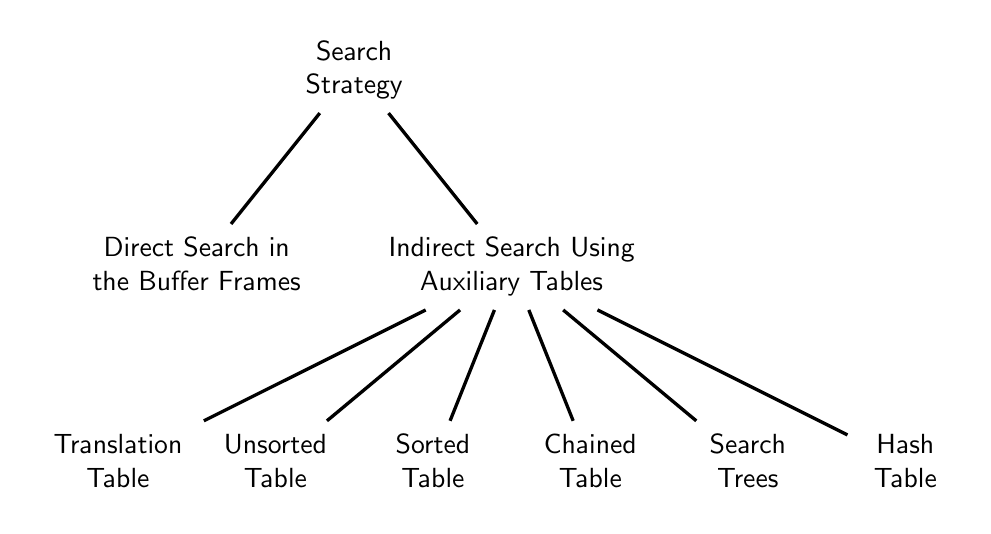
\begin{tikzpicture}[]
				\node[]								(algorithms)		[]		{\begin{tabular}{c}Search\\Strategy\end{tabular}}
					child {node[]						(seq)				[]		{\begin{tabular}{c}Direct Search in\\the Buffer Frames\end{tabular}}}
					child {node[]						(aux)				[]		{\begin{tabular}{c}Indirect Search Using\\Auxiliary Tables\end{tabular}}
						child {node[]					(trans)			[]		{\begin{tabular}{c}Translation\\Table\end{tabular}}}
 						child {node[]					(unsort)			[]		{\begin{tabular}{c}Unsorted\\Table\end{tabular}}}
 						child {node[]					(sort)				[]		{\begin{tabular}{c}Sorted\\Table\end{tabular}}}
						child {node[]					(chain)			[]		{\begin{tabular}{c}Chained\\Table\end{tabular}}}
						child {node[]					(tree)			[]		{\begin{tabular}{c}Search\\Trees\end{tabular}}}
						child {node[]					(hash)			[]		{\begin{tabular}{c}Hash\\Table\end{tabular}}}
				};
		
			\end{tikzpicture}
		}
        \vspace{.5em}
		\caption[Classification of buffer frame search strategies]{Classification of search strategies to translate from page IDs to buffer frame IDs as in \cite{Effelsberg:1984}}
		\label{fig:locate}
	\end{figure}
\end{@empty}
	
	The following overview of costs caused by those search strategies leads to the result that the usage of a \emph{hash table} is the preferred strategy. Let $n = \text{number of buffer pool frames}$ and $p = \text{total number of pages}$:
	\begin{itemize}
		\item	\textbf{Direct Search in Buffer Frames:} $T_{\text{avg}}^{\text{search}} \in \mathcal O\left(\frac{n}{2}\right)$, $T_{\text{worst}}^{\text{search}} \in  \mathcal O\left(n\right)$ (Swapping can be expensive using virtual memory management)
		\item	\textbf{Translation Table:} $T^{\text{search}} \in  \mathcal O\left(1\right)$, $T^{\text{insert}} \in  \mathcal O\left(1\right)$, $S\text{\tiny{pace}} \in \mathcal O\left(p\right)$
		\item	\textbf{Unsorted Table:} $T_{\text{avg}}^{\text{search}} \in  \mathcal O\left(\frac{n}{2}\right)$, $T_{\text{worst}}^{\text{search}} \in  \mathcal O\left(n\right)$
		\item	\textbf{Sorted Table:} $T_{\text{avg}}^{\text{search}} \in  \mathcal O\left(\log_2n\right)$, $T_{\text{avg}}^{\text{insert}} \in  \mathcal O\left(n\log_2n\right)$
		\item	\textbf{Chained Table:} $T_{\text{avg}}^{\text{search}} \in  \mathcal O\left(\log_2n\right)$, $T_{\text{avg}}^{\text{insert}} \in  \mathcal O\left(\log_2n\right)$
		\item	\textbf{Search Trees:} $T_{\text{avg}}^{\text{search}} \in  \mathcal O\left(\log n\right)$, $T_{\text{avg}}^{\text{insert}} \in  \mathcal O\left(\log n\right)$
		\item	\textbf{Hash Table:} $T_{\text{avg}}^{\text{search}} \in  \mathcal O\left(1\right)$, $T_{\text{avg}}^{\text{insert}} \in  \mathcal O\left(1\right)$, $T_{\text{worst}}^{\text{search}} \in  \mathcal O\left(n\right)$
	\end{itemize}
	The \emph{direct search in the buffer frames} reads the page ID within each page residing in the buffer pool and therefore it needs to access each buffer pool frame. If the main memory is managed using virtual memory management, the access to wide-spread memory addresses could cause a notable overhead due to swapping.
	
	The \emph{translation table} stores per page ID the frame ID where the corresponding page can be found in the buffer pool. Therefore the entry of each page not residing in the buffer pool will be empty (null).
	
	The \emph{unsorted table} would typically use the addressing of the buffer frames and it would store for each buffer frame ID the page ID of the contained frame. While it works similar to the direct search in the buffer frames, it doesn't require the access to wide-spread memory addresses.

\begin{@empty}
	\tikzset{%
		table/.style = {draw = black, shape = rectangle split, rectangle split parts = 9, rectangle split horizontal, font = \bfseries}
	}

	\begin{figure}[ht!]
		\centering
		\resizebox{\textwidth}{!}{
			\begin{tikzpicture}
				\node[table]	(table)	{\nodepart{one}7785\nodepart{two}6977\nodepart{three}4347\nodepart{four}3380\nodepart{five}5610\nodepart{six}6376\nodepart{seven}4877\nodepart{eight}3332\nodepart{nine}3354};
				
				\foreach \anchor/\address in {one/0, two/1, three/2, four/3, five/4, six/5, seven/6, eight/7, nine/8} {
					\node[]	(\address)		[above = .375cm of table.\anchor]	{\address};
				}
			\end{tikzpicture}
		}
        \vspace{.5em}
		\caption{An unsorted table used to map buffer frames to page IDs.}
		\label{fig:unsortedTable}
	\end{figure}
\end{@empty}
	
	The \emph{sorted table} contains an entry for each used buffer frame sorted by the page ID of the contained page. It allows binary searching but the insertion requires sorting and therefore serious movement of entries inside the table is required.

\begin{@empty}
	\tikzset{%
		table/.style = {draw = black, shape = rectangle split, rectangle split parts = 9, rectangle split horizontal, font = \bfseries, inner xsep = -2pt, inner ysep = 0pt}
	}

	\begin{figure}[ht!]
		\centering
		\resizebox{\textwidth}{!}{
			\begin{tikzpicture}
				\node[table]	(table)	{\nodepart{nine}\begin{tabular}{c}7785 \\ $\rightarrow$ 0\end{tabular}
									\nodepart{eight}\begin{tabular}{c}6977 \\ $\rightarrow$ 1\end{tabular}
									\nodepart{four}\begin{tabular}{c}4347 \\ $\rightarrow$ 2\end{tabular}
									\nodepart{three}\begin{tabular}{c}3380 \\ $\rightarrow$ 3\end{tabular}
									\nodepart{six}\begin{tabular}{c}5610 \\ $\rightarrow$ 4\end{tabular}
									\nodepart{seven}\begin{tabular}{c}6376 \\ $\rightarrow$ 5\end{tabular}
									\nodepart{five}\begin{tabular}{c}4877 \\ $\rightarrow$ 6\end{tabular}
									\nodepart{one}\begin{tabular}{c}3332 \\ $\rightarrow$ 7\end{tabular}
									\nodepart{two}\begin{tabular}{c}3354 \\ $\rightarrow$ 8\end{tabular}};
			\end{tikzpicture}
		}
        \vspace{.5em}
		\caption{A sorted table used to map page IDs to buffer frames.}
		\label{fig:sortedTable}
	\end{figure}
\end{@empty}
	
	The entries of a \emph{chained table} are similar to those of the sorted table. But instead of ordering the entries using their memory addresses (e.g. using an array) inside the table, the entries are chained using pointers from one entry to the next\footnote[1]{With regard to the ordering on the page IDs.} (and its previous) and an insert or removal only requires to connect the previous and the next entry of the removed entry and to search the new position for insertion. It has some disadvantage against a sorted table with regard to binary search but the insertion works much faster.

\begin{@empty}
	\tikzset{%
		node distance = .25cm,
		node/.style = {draw = black, shape = rectangle split, rectangle split parts = 2, font = \bfseries, inner xsep = -2pt, inner ysep = 0pt}
	}

	\begin{figure}[ht!]
		\centering
		\resizebox{\textwidth}{!}{
			\begin{tikzpicture}
				\node[node]	(node0)	[]				{\nodepart{one}\vphantom{M}\nodepart{two}\begin{tabular}{c}3332 \\ $\rightarrow$ 7\end{tabular}};
				\node[node]	(node1)	[right = of node0]	{\nodepart{one}\vphantom{M}\nodepart{two}\begin{tabular}{c}3354 \\ $\rightarrow$ 8\end{tabular}};
				\node[node]	(node2)	[right = of node1]	{\nodepart{one}\vphantom{M}\nodepart{two}\begin{tabular}{c}3380 \\ $\rightarrow$ 3\end{tabular}};
				\node[node]	(node3)	[right = of node2]	{\nodepart{one}\vphantom{M}\nodepart{two}\begin{tabular}{c}4347 \\ $\rightarrow$ 2\end{tabular}};
				\node[node]	(node4)	[right = of node3]	{\nodepart{one}\vphantom{M}\nodepart{two}\begin{tabular}{c}4877 \\ $\rightarrow$ 6\end{tabular}};
				\node[node]	(node5)	[right = of node4]	{\nodepart{one}\vphantom{M}\nodepart{two}\begin{tabular}{c}5610 \\ $\rightarrow$ 4\end{tabular}};
				\node[node]	(node6)	[right = of node5]	{\nodepart{one}\vphantom{M}\nodepart{two}\begin{tabular}{c}6376 \\ $\rightarrow$ 5\end{tabular}};
				\node[node]	(node7)	[right = of node6]	{\nodepart{one}\vphantom{M}\nodepart{two}\begin{tabular}{c}6977 \\ $\rightarrow$ 1\end{tabular}};
				\node[node]	(node8)	[right = of node7]	{\nodepart{one}\vphantom{M}$\cdot$\nodepart{two}\begin{tabular}{c}7785 \\ $\rightarrow$ 0\end{tabular}};
				
				\foreach \this/\next in {0/1, 1/2, 2/3, 3/4, 4/5, 5/6, 6/7, 7/8} {
					\draw[ -> ]		([yshift = 1pt] node\this.mid)	to [bend left = 12.5]		(node\next.text west);
				}
			\end{tikzpicture}
		}
        \vspace{.5em}
		\caption{A chained table used to map page IDs to buffer frames.}
		\label{fig:chainedTable}
	\end{figure}
\end{@empty}
	
	There are numerous \emph{search tree} structures like AVL-trees or red–black trees and therefore I refer to \cite{Knuth:1998} for further details on them. All those tree structures share a similar asymptotic complexity for the average cases but they have different worst case behaviour (and different worst cases). In this application, the search key will be the page ID of pages cached in the buffer pool and the entries will contain the buffer frame IDs where the corresponding page is located at.
	
\begin{@empty}
	\tikzset{%
		node distance = .5cm,
		bucketHeaderNumber/.style = {shape = rectangle, draw = black, minimum width = .1\textwidth, anchor = south west, minimum height = .5cm, font = \bfseries},
		bucketHeaderNext/.style = {shape = rectangle, draw = black, minimum width = .1\textwidth, anchor = south east, minimum height = .5cm},
		bucketBody/.style = {shape = rectangle split, rectangle split parts = #1, draw = black, minimum width = .2\textwidth, anchor = north},
		pid/.style = {draw = none, font = \bfseries},
		hashFunction/.style = {draw = black, shape = rectangle, rounded corners = 5pt, minimum height = .55\textheight, minimum width = .125\textwidth},
		hashFunctionText/.style = {font = \bfseries}
	}

	\nottoggle{bwmode}{
		\tikzset{%
			hashFunction/.append style = {draw = ForestGreen, fill = ForestGreen!15}, 
			hashFunctionText/.append style = {text = ForestGreen},
			bucketHeaderNumber/.append style = {draw = Purple, fill = Purple!15},
			bucketHeaderNext/.append style = {draw = Purple!75, fill = Purple!11.25},
		}
	}

	\begin{figure}[ht!]
		\centering
		\scalebox{1}{
			\begin{tikzpicture}
				
				% Create the hash function:
				\node[hashFunction]				(func)		[]						{};
				\node[hashFunctionText]			(funcText)		[below = .025cm of func.north]	{$\bm{\text{mod } 5}$};
				
				% Create the hashed Page IDs:
				\pgfmathsetseed{2144}
				\pgfmathsetmacro{\numOfPages}{4}
				\pgfmathsetmacro{\initialValue}{int(10000 * rand)}
				\ifthenelse{\initialValue < 0}{
					\pgfmathsetmacro{\initialValue}{int(-1 * \initialValue)}
				}{}
				\node[pid]							(pid0)		[left = of func]			{\initialValue};
				\node[]							(help0)		[right = of pid0]			{};
				\draw[]		(pid0.east)	--		(help0.west);
				\foreach \x in {1, ..., \numOfPages}{
					\ifthenelse{\x = 1}{
						\pgfmathtruncatemacro{\previousTop}{0}
						\pgfmathtruncatemacro{\previousBottom}{0}
					}{
						\pgfmathtruncatemacro{\previousTop}{(2 * \x) - 3}
						\pgfmathtruncatemacro{\previousBottom}{(2 * \x) - 2}
					}
					\pgfmathtruncatemacro{\top}{(2 * \x) - 1}
					\pgfmathtruncatemacro{\bottom}{(2 * \x)}
					\pgfmathsetmacro{\topValue}{int(10000 * rand)}
					\pgfmathsetmacro{\bottomValue}{int(10000 * rand)}
					\ifthenelse{\topValue < 0}{
						\pgfmathsetmacro{\topValue}{int(-1 * \topValue)}
					}{}
					\ifthenelse{\bottomValue < 0}{
						\pgfmathsetmacro{\bottomValue}{int(-1 * \bottomValue)}
					}{}
					
					\node[pid]							(pid\top)			[above = of pid\previousTop]			{\topValue};
					\node[]							(help\top)			[right = of pid\top]					{};
					\draw[]		(pid\top.east)	--		(help\top.west);
					\node[pid]							(pid\bottom)		[below = of pid\previousBottom]			{\bottomValue};
					\node[]							(help\bottom)		[right = of pid\bottom]				{};
					\draw[]		(pid\bottom)	--		(help\bottom);
				}
				
				% Create the hash buckets:
				\pgfmathsetmacro{\numOfBuckets}{2}
				\pgfmathsetmacro{\initialBucket}{int(\numOfBuckets)}
				\node[bucketBody=2]				(bucketBody2)		[right = of func, yshift = -.25cm]			{\nodepart{one}$4347 \rightarrow 2$\nodepart{two}$4877 \rightarrow 6$};
				\node[bucketBody=2]				(bucketBody1)		[above = 1cm of bucketBody2]			{\nodepart{one}$6376 \rightarrow 5$\nodepart{two}$\cdot$};
				\node[bucketBody=2]				(bucketBody3)		[below = 1cm of bucketBody2]			{\nodepart{one}$\cdot$\nodepart{two}$\cdot$};
				\node[bucketBody=2]				(bucketBody0)		[above = 1cm of bucketBody1]			{\nodepart{one}$3380 \rightarrow 3$\nodepart{two}$5610 \rightarrow 4$};
				\node[bucketBody=2]				(bucketBody4)		[below = 1cm of bucketBody3]			{\nodepart{one}$3354 \rightarrow 8$\nodepart{two}$\cdot$};
				\node[bucketHeaderNumber]		at (bucketBody0.north west)	(bucketHeaderNu0)	[]			{0};
				\node[bucketHeaderNext]			at (bucketBody0.north east)	(bucketHeaderNe0)	[]			{};
				\node[bucketHeaderNumber]		at (bucketBody1.north west)	(bucketHeaderNu1)	[]			{1};
				\node[bucketHeaderNext]			at (bucketBody1.north east)	(bucketHeaderNe1)	[]			{$\cdot$};
				\node[bucketHeaderNumber]		at (bucketBody2.north west)	(bucketHeaderNu2)	[]			{2};
				\node[bucketHeaderNext]			at (bucketBody2.north east)	(bucketHeaderNe2)	[]			{};
				\node[bucketHeaderNumber]		at (bucketBody3.north west)	(bucketHeaderNu3)	[]			{3};
				\node[bucketHeaderNext]			at (bucketBody3.north east)	(bucketHeaderNe3)	[]			{$\cdot$};
				\node[bucketHeaderNumber]		at (bucketBody4.north west)	(bucketHeaderNu4)	[]			{4};
				\node[bucketHeaderNext]			at (bucketBody4.north east)	(bucketHeaderNe4)	[]			{$\cdot$};
				\node[]							(bucketHelp0)		[left = of bucketHeaderNu0]			{};
				\node[]							(bucketHelp1)		[left = of bucketHeaderNu1]			{};
				\node[]							(bucketHelp2)		[left = of bucketHeaderNu2]			{};
				\node[]							(bucketHelp3)		[left = of bucketHeaderNu3]			{};
				\node[]							(bucketHelp4)		[left = of bucketHeaderNu4]			{};
				\draw[]		(bucketHeaderNu0.west)	--		(bucketHelp0.east);
				\draw[]		(bucketHeaderNu1.west)	--		(bucketHelp1.east);
				\draw[]		(bucketHeaderNu2.west)	--		(bucketHelp2.east);
				\draw[]		(bucketHeaderNu4.west)	--		(bucketHelp4.east);

				\node[bucketBody=4]				(bucketBody00)		[right = of bucketBody0, yshift = -.325cm]			{\nodepart{one}$7785 \rightarrow 0$\nodepart{two}$\cdot$\nodepart{three}$\cdot$\nodepart{four}$\cdot$};
				\node[bucketHeaderNumber]		at (bucketBody00.north west)	(bucketHeaderNu00)	[]			{0};
				\node[bucketHeaderNext]			at (bucketBody00.north east)	(bucketHeaderNe00)	[]			{$\cdot$};
				\draw[]		(bucketHeaderNe0.center)	--		(bucketHeaderNu00.west);

				\node[bucketBody=4]				(bucketBody20)		[right = of bucketBody2, yshift = -.41cm]			{\nodepart{one}$3332 \rightarrow 7$\nodepart{two}$6977 \rightarrow 1$\nodepart{three}$\cdot$\nodepart{four}$\cdot$};
				\node[bucketHeaderNumber]		at (bucketBody20.north west)	(bucketHeaderNu20)	[]			{2};
				\node[bucketHeaderNext]			at (bucketBody20.north east)	(bucketHeaderNe20)	[]			{$\cdot$};
				\draw[]		(bucketHeaderNe2.center)	--		(bucketHeaderNu20.west);

				\draw[]		(help5.west)	--		(bucketHelp0.east);
				\draw[]		(help1.west)	--		(bucketHelp0.east);
				\draw[]		(help8.west)	--		(bucketHelp0.east);
				\draw[]		(help4.west)	--		(bucketHelp1.east);
				\draw[]		(help7.west)	--		(bucketHelp2.east);
				\draw[]		(help3.west)	--		(bucketHelp2.east);
				\draw[]		(help0.west)	--		(bucketHelp2.east);
				\draw[]		(help6.west)	--		(bucketHelp2.east);
				\draw[]		(help2.west)	--		(bucketHelp4.east);
			\end{tikzpicture}
		}
        \vspace{.5em}
		\caption[Typical hash table design]{Typical design of a hash table. It maps a page ID of a page in the buffer pool (left) using a hash function (center) to a hash bucket (right). A hash bucket contains an entry for each page ID currently mapped to it but if the hash bucket is full (two entries possible in this example), a chained hash bucket (far right) will be used. Each entry maps a page ID to a buffer frame ID where the corresponding page can be found. The used test bed \emph{Zero} uses an implementation based on this concept.}
		\label{fig:hashtable}
	\end{figure}
\end{@empty}

	A \emph{hash table} uses the page ID as key as well. This key is mapped to a smaller address space and each value of this address space corresponds to a hash bucket which is used to store the entries in it. There are numerous concepts on the exact mechanics of such a data structure and therefore I'll refer again to \cite{Knuth:1998}. Like before, the asymptotic complexity for the average cases of those concepts is similar and therefore the selection of a specific implementation depends on numerous assumptions which are of the scope of this thesis. As mentioned before, the auxiliary structures of the buffer pool are accessed concurrently and therefore a data structure which takes that into account is preferable. And such concurrent hash tables (also called hash maps) are still an active topic of research (and development) \cite{JunctionLibrary}. An exemplary concept of an hash table is shown in figure \ref{fig:hashtable}.
	
\begin{@empty}
	\tikzset{%
		node distance = 1cm,
		startstop/.style = {rectangle, rounded corners, minimum width = 4cm, text width = 6cm, align = center},
		io/.style = {trapezium, trapezium left angle = 70, trapezium right angle = 110, minimum width = 4cm, text width = 4cm, align = center},
		process/.style = {rectangle, minimum width = 4cm, text width = 6cm, align = center},
		decision/.style = {diamond, aspect=2, minimum width = 8cm, text width = 6cm, align = center, inner sep = -3pt},
		arrow/.style = { -> , thick, >=stealth}
	}

	\nottoggle{bwmode}{
		\tikzset{%
			startstop/.append style = {draw = red, fill = red!15}, 
			io/.append style = {draw = blue, fill = blue!15},
			process/.append style = {draw = orange, fill = orange!15},
			decision/.append style = {draw = green, fill = green!15},
		}
	}{
		\tikzset{%
			startstop/.append style = {draw = black}, 
			io/.append style = {draw = black},
			process/.append style = {draw = black},
			decision/.append style = {draw = black}
		}
	}

	\begin{figure}[ht!]
		\centering
		\scalebox{.7}{
			\begin{tikzpicture}
				\node[]						(center start)		[]						{};
				\node[io]						(page)			[above = .35cm of center start]	{Buffer pool page image};
				\node[io]						(key)				[below = .35cm of center start]	{Search key};
				\node[process]					(search)			[right = 5cm of center start]	{Look for entry in page image that corresponds to search key};
				\node[decision]					(found1)			[below = of search]			{Found entry?};
				\node[startstop]					(miss)			[below = of found1]			{Search key not found};
				\node[process]					(get id)			[left= of found1]				{Get identifier of the next page to search from the page image};
				\node[process]					(hash)			[below = of get id]			{calculate hash id of the page id};
				\node[process]					(lookup)			[below = of hash]			{Look in buffer pool hash table for hashed page id (protect hash table)};
				\node[decision]					(found2)			[below = of lookup]			{Found hashed page id?};
				\node[startstop]					(final)			[right = of found2]			{Return buffer pool page image of the next page to search};
				\node[process]					(load)			[above = of final]			{Bring page into buffer pool (possibly need to evict another page image)};

				\draw[arrow]	(page)			|-						(search);
				\draw[arrow]	(key)				|-						(search);
				\draw[arrow]	(search)			--						(found1);
				\draw[arrow]	(found1)			--	node[right]	{no}		(miss);
				\draw[arrow]	(found1)			--	node[above]	{yes}		(get id);
				\draw[arrow]	(get id)			--						(hash);
				\draw[arrow]	(hash)			--						(lookup);
				\draw[arrow]	(lookup)			--						(found2);
				\draw[arrow]	(found2)			--	node[above left]	{no}	(load.west);
				\draw[arrow]	(found2)			--	node[above]		{yes}	(final);
				\draw[arrow]	(load)			--						(final);
			\end{tikzpicture}
		}
        \vspace{.5em}
		\caption[Control flow of fixing a page without pointer swizzling]{The control flow of fixing a page given a search key and an index page when a hash table is used to locate pages in the buffer pool. This summarizing diagram is taken from \cite{Graefe:2014}.}
		\label{fig:locatehash}
	\end{figure}
\end{@empty}

\subsection[With Pointer Swizzling]{Locate Pages in the Buffer Pool with Pointer Swizzling} \label{subsec:conceptbufferswizzling}

	Following \emph{Moore's Law}, the price of memory rapidly decreases as some actual data in figure \ref{fig:memorycost} point out. Therefore the available \emph{memory capacity increases exponentially} by time. As a result of that trend, there are many OLTP applications where the whole working set (or even the whole database) fits in the buffer pool.
	
	In such a case, the performance of a page hit defines the overall performance of the buffer pool as there won't be many page misses anymore when the whole working set is cached in main memory. Therefore the optimization of page hits is a major concern. The only slow operation performed during a page hit is the searching of the appropriate buffer frame (the concurrency control might delay a transaction as well). Even the usage of a \emph{hash table} which in average searches in $\mathcal{O}\left(1\right)$ needs a reasonable number of instruction cycles to perform it's operations. To search a page in the buffer pool, the calculation of the hash value using the hash function is required. Afterwards, the corresponding hash bucket needs to be scanned until the searched for page is found. If that page cannot be found, an arbitrary number ($\mathcal{O}\left(n\right)$) of chained hash buckets needs to be scanned as well until the page is found or until a page miss is detected. And that worst-case performance of those \emph{hash tables} is in $\mathcal{O}\left(n\right)$ which cannot be tolerated.

\begin{@empty}
	\tikzset{%
		dataPoints/.style = {only marks, mark = x},
		trend/.style = {thick},
	}

	\nottoggle{bwmode}{
		\tikzset{%
			dataPoints/.append style = {color = blue},
			trend/.append style = {color = red},
		}
	}
	
	\begin{figure}[ht!]
		\centering
		\resizebox{\textwidth}{!}{
			\begin{tikzpicture}
				\begin{axis}[xlabel = {$\text{Time }\left[\si{\year}\right]$},
						   xmin = 1957,
						   xmax = 2020,
						   xtick = {1960, 1965, ..., 2020},
						   xticklabels = {1960, 1965, ..., 2020},
						   minor x tick num = 4,
						   ylabel = {$\text{Memory Price }\left[\si{\usdollar\per\mebi\byte}\right]$},
						   ymax = 500000000,
						   ymode = log,
						   scaled y ticks = false,
						   grid = major,
						   width = 1.5\textwidth,
						   height = .75\textheight]		

					\addplot[dataPoints] table {./tex/data/memory_prices.csv};
					\addplot[trend] table[y = {create col/linear regression = {y = price}}] {./tex/data/memory_prices.csv};
				\end{axis}
			\end{tikzpicture}
		}
        \vspace{.25em}
		\caption[History of memory prices]{History of memory prices\footnotemark}
		\label{fig:memorycost}
	\end{figure}
\end{@empty}

    \footnotetext{\url{https://hblok.net/blog/storage/}}

	Many applications suffer from this overhead when locating persistent objects cached in main memory. In general, applications like \textit{persistent programming languages}, \textit{database programming languages}, \textit{object oriented database systems}, \textit{persistent object stores} or \textit{object servers} work on persistent objects stored on secondary storage. But the same reasons why a buffer pool is used in DBMS also hold for the need of an object cache in those applications. Generally, those applications use unique object identifiers to reference persistent objects and therefore it's needed to translate this address to a memory address during an object reference. To eliminate this overhead, \emph{pointer swizzling} was introduced in the late 80's and classified in \cite{White:1995}. \emph{To swizzle a pointer means to transform the address of the persistent object referenced there to a more direct address of the transient object in a way that this transformation could be used during multiple indirections of this pointer} \cite{Moss:1992}. White and DeWitt identified \emph{7 dimensions} on which different approaches of pointer swizzling can be characterized. The classification of the pointer swizzling approach for the DBMS buffer pool proposed by Graefe et al. in \cite{Graefe:2014} is shown in figure \ref{fig:cassification}.
	
\begin{@empty}
	\tikzset{%
		selected/.style = {font = \bfseries, very thick}
	}

	\nottoggle{bwmode}{
		\tikzset{%
			selected/.append style = {text = blue, color = blue}
		}
	}
	
	\begin{figure}[ht!]
		\centering
		\scalebox{1}{
			\begin{tikzpicture}
				\draw arc [start angle = 0,   
                 				end angle = 360,
                					x radius = 4cm, 
                 				y radius = 4cm]
							node [pos = 1 * 1/14]				(eager)		{eager}
							node [pos = 2 * 1/14, selected]		(direct)		{direct}
							node [pos = 3 * 1/14, selected]		(in-place)		{in-place}
							node [pos = 4 * 1/14]				(hardware)	{hardware}
							node [pos = 5 * 1/14]				(no-swizzling)	{no-swizzling}
							node [pos = 6 * 1/14]				(no uncaching)	{no uncaching}
							node [pos = 7 * 1/14]				(partial)		{partial}
							node [pos = 8 * 1/14, selected]		(lazy)		{lazy}
							node [pos = 9 * 1/14]				(indirect)		{indirect}
							node [pos = 10 * 1/14]			(copy)		{copy}
							node [pos = 11 * 1/14, selected]	(software)		{software}
							node [pos = 12 * 1/14, selected]	(swizzling)		{swizzling}
							node [pos = 13 * 1/14, selected]	(uncaching)	{uncaching}
							node [pos = 14 * 1/14, selected]	(full)			{full};
				
					\node[anchor = center, right = 4cm of partial.center]			(center)			{};
					\path[->]	
						(center.center)		edge[selected]		(direct)
						(center.center)		edge[]			(indirect)
						(center.center)		edge[selected]		(in-place)
						(center.center)		edge[]			(copy)
						(center.center)		edge[]			(hardware)
						(center.center)		edge[selected]		(software)
						(center.center)		edge[]			(partial)
						(center.center)		edge[selected]		(full)
						(center.center)		edge[]			(no-swizzling)
						(center.center)		edge[selected]		(swizzling)
						(center.center)		edge[]			(eager)
						(center.center)		edge[selected]		(lazy)
						(center.center)		edge[]			(no uncaching)
						(center.center)		edge[selected]		(uncaching);
				\end{tikzpicture}
			}
        \vspace{.25em}
		\caption[Dimensions of pointer swizzling]{Dimensions of pointer swizzling as of \cite{White:1995} and the classification of the presented approach}
		\label{fig:cassification}
	\end{figure}
\end{@empty}

	The approach of using pointer swizzling in the buffer pool of a DBMS obviously uses \emph{swizzling}.
	
	As a DBMS typically cannot use hardware acceleration, the swizzling and unswizzling of references in done in \emph{software}.
	
	The buffer pool's addressing unit is the page and therefore those are the persistent objects that needs to be concerned by the pointer swizzling approach. The references that are swizzled are the page identifiers. The proposed approach of pointer swizzling inside the buffer pool only allows a primary Foster B-tree index \cite{Graefe:2012} on the database and therefore there exists only one pointer to each page. Those pointers are always swizzled when the referenced child page also resides in main memory. The pointers to the root pages of the Foster B-tree are stored separately and those got also swizzled. As the buffer pool doesn't omit the swizzling of some of the pointers it knows, the approach is \emph{full} swizzling.
	
	As a collection (e.g. a table) in a DBMS can be much larger than the buffer pool, it's not always possible to load a whole collection which is indexed in one Foster B-tree into the main memory. Therefore the proposed approach cannot use eager but \emph{lazy} swizzling. This means that only a subset of the pointers, inside a page which is cached in the buffer pool, need to be swizzled. Eager swizzling would require the swizzling of all the page IDs inside pages that a in the buffer pool. This would require that all those pages are also available in the buffer pool. An hierarchical index structure like a Foster B-tree would therefore cause an eager loading of the pages where all the pages that are part of the index structure are loaded into main memory when the root gets accessed. But as lazy swizzling allows a page pointer inside a buffered page to be not swizzled, it's unclear during the dereferencing of such a pointer, if it's a page hit (pointer is swizzled and therefore a memory address) or if it's a page miss (pointer is a page ID and the page needs to be requested from the storage management). This additional check of the semantics of a discovered pointer adds some overhead. In the proposed approach, each swizzled pointer has set a bit that is never set in valid page IDs. Therefore the check only requires the checking if this bit is set and the unsetting of this bit to receive the memory address of the referenced page. The tradeoff of this approach is the additional bit needed in every pointer that cannot be used to extend the possible number of pages in the DBMS but the usage of \SI{64}{\bit} architectures in modern computer systems makes this drawback negligible.
	
	An approach that would allow eager swizzling in the buffer pool would need to use indirect swizzling. This would introduce an so called object table entry. With indirect swizzling, a swizzled pointer points to such an object table entry and this entry contains the actual address of the referenced page. Therefore this additional indirection allows eager swizzling where only the object table entries for referenced pages are created when a page gets loaded in main memory. Those object table entries will contain the page ID or the memory address of the corresponding page. But the proposed approach uses \emph{direct} swizzling and therefore there is no indirection during a page reference when the pointer is swizzled.
	
	The pointers are swizzled \emph{in-place} and therefore there isn't another copy of the page in main memory not containing swizzled pointers. But the definition of copy and in-place swizzling cannot be fully applied to the given approach as the classification using this dimension requires a distinction between a buffer pool containing pages and an object cache containing objects. Copy swizzling would require a single accessed object to be copied from the page into the object cache. The cached page would still contain the object without the pointers being swizzled (unswizzling not required when page is written to secondary storage) while an accessed object from that page would be copied to the object cache where the pointers are swizzled pointing to referenced objects.
	
	The proposed approach of pointer swizzling in the DBMS buffer pool allows \emph{uncaching}. Therefore a page that doesn't contain a swizzled pointer can be evicted from the buffer pool. Those pages are the leafs of the subset of the Foster B-tree cached in the buffer pool. The eviction of pages containing swizzled pointers would make the approach more complex. The eviction of a page would require the unswizzling of all the contained pointers to allow the writing of the page. It would also require the check if the parent page actually resides in main memory and therefore it would be possible that an eviction doesn't imply the unswizzling of a pointer. Another possible problem would be the situation where there isn't a pointer to a page that resides in the buffer pool. When the evicted parent page gets loaded into the buffer pool again while the child still resides in the buffer pool, the pointer in the parent page would still be not swizzled and therefore a future reference of the child page would require the usage of a hash table to locate the page even when a page hit happens. This would also require the swizzling of a pointer to a page that was loaded to the buffer pool before the pointer to it was loaded to the buffer pool. But the major reason for this decision is the fact that a page cannot be accessed without using its parent page as there only exists one pointer per page. It wouldn't make sense to hold a page in the buffer pool when the parent page was evicted. An access of the page would require the parent page to be loaded to the buffer pool again and due to the hierarchical structure of the pages, the parent page has a higher probability of being used.
	
	The simplicity of the proposed approach can be seen in figure \ref{fig:locateswizzle}.

\begin{@empty}
	\tikzset{%
		node distance = 1cm,
		startstop/.style = {rectangle, rounded corners, minimum width = 4cm, text width = 6cm, align = center},
		io/.style = {trapezium, trapezium left angle = 70, trapezium right angle = 110, minimum width = 4cm, text width = 4cm, align = center},
		process/.style = {rectangle, minimum width = 4cm, text width = 6cm, align = center},
		decision/.style = {diamond, aspect=2, minimum width = 8cm, text width = 6cm, align = center, inner sep = -3pt},
		arrow/.style = { -> , thick, >=stealth}
	}

	\nottoggle{bwmode}{
		\tikzset{%
			startstop/.append style = {draw = red, fill = red!15}, 
			io/.append style = {draw = blue, fill = blue!15},
			process/.append style = {draw = orange, fill = orange!15},
			decision/.append style = {draw = green, fill = green!15}
		}
	}{
		\tikzset{%
			startstop/.append style = {draw = black}, 
			io/.append style = {draw = black},
			process/.append style = {draw = black},
			decision/.append style = {draw = black}
		}
	}

	\begin{figure}[ht!]
		\centering
		\resizebox{\textwidth}{!}{
			\begin{tikzpicture}
				\node[]						(center start)		[]						{};
				\node[io]						(page)			[above = .35cm of center start]	{Buffer pool page image};
				\node[io]						(key)				[below = .35cm of center start]	{Search key};
				\node[process]					(search)			[right = 5cm of center start]	{Look for entry in page image that corresponds to search key};
				\node[decision]					(found)			[below = of search]			{Found entry?};
				\node[startstop]					(miss)			[below = of found]			{Search key not found};
				\node[process]					(get id)			[left = of found]				{Get identifier of the next page to search from the page image};
				\node[decision]					(swizzled)			[below = of get id]			{Identifier swizzled?};
				\node[process]					(load)			[below = of swizzled]			{Bring page into buffer pool (possibly need to evict another  page image) and swizzle pointer on it};
				\node[startstop]					(final)			[right = 1.875cm of load]		{Return buffer pool page image of the next page to search};

				\draw[arrow]	(page)			|-						(search);
				\draw[arrow]	(key)				|-						(search);
				\draw[arrow]	(search)			--						(found);
				\draw[arrow]	(found)			--	node[right]		{no}	(miss);
				\draw[arrow]	(found)			--	node[above]		{yes}	(get id);
				\draw[arrow]	(get id)			--						(swizzled);
				\draw[arrow]	(swizzled)			--	node[right]		{no}	(load);
				\draw[arrow]	(swizzled)			--	node[above right]	{yes}	(final);
				\draw[arrow]	(load)			--						(final);
			\end{tikzpicture}
		}
        \vspace{.5em}
		\caption[Control flow of fixing a page with pointer swizzling]{The control flow of fixing a page given a search key and an index page when pointer swizzling is used to locate pages in the buffer pool. This summarizing diagram is taken from \cite{Graefe:2014}.}
		\label{fig:locateswizzle}
	\end{figure}
\end{@empty}
	
\section[Design and Implementation of the Buffer Manager]{Design and Implementation of the DBMS Buffer Management as in \cite{Graefe:2014}}

\subsection[\emph{Zero} - The Test Bed]{\emph{Zero} - A Test Bed for DBMS Techniques}

	To illustrate the acceleration of a DBMS when enabling pointer swizzling inside the buffer management as described in subsection \ref{subsec:conceptbufferswizzling}, Goetz Graefe et al. used the transactional storage manager \emph{Zero} where they introduced the technique.
	
\subsubsection[History of \emph{Zero}]{The History of \emph{Zero}}
	
	\emph{Zero}\footnote{\url{https://github.com/caetanosauer/zero}}, that gets developed by Goetz Graefe's research group at \emph{HP Labs} and the \emph{Database and Information Systems Group} at the \emph{University of Kaiserslautern}, is a fork of the \emph{Shore-MT Storage Manager}\footnote{\url{https://sites.google.com/site/shoremt/}}(short for ``\textbf{Shore} Storage Manager: The \textbf{M}ulti-\textbf{T}hreaded Version''), which is, as the name suggests the successor of the \emph{Shore Storage Manager}\footnote{\url{http://research.cs.wisc.edu/shore/}} (acronym for ``\textbf{S}calable \textbf{H}eterogeneous \textbf{O}bject \textbf{RE}pository''). \emph{Shore-MT} has been developed at the \emph{Carnegie Mellon University} and \emph{École polytechnique fédérale de Lausanne} since the mid 2000's whereas \emph{Shore}'s development started in the early 1990's at the \emph{University of Wisconsin}. Originally \emph{Shore}\addtocounter{footnote}{-1}\footnotemark (included a whole DBMS but only the development of the storage manager continued till the time when the development of \emph{Shore-MT} started, which is as well only a storage manager. Back in the mid 1990's there was even a predecessor of \emph{Shore}, \emph{EXODUS}\footnote{\url{http://research.cs.wisc.edu/exodus/}} (acronym for ``\textbf{EX}tensible \textbf{O}bject-Oriented \textbf{D}atabase \textbf{S}ystem Toolkit'', the ``\textbf{U}'' has no meaning) which was a research project at the \emph{University of Wisconsin} funded by the \emph{ARPA} (also known as \emph{DARPA}).
	
	Figure \ref{fig:testbedhistory} gives an overview on the development (based on new releases of the software or publications about software for the case that a version history is unavailable) of these database management system prototypes.
	
	\tikzset{%
		every node/.style = {font = \sffamily},
		year/.style = {draw = none, anchor = west, rotate = -90, outer sep = .1em},
		softwarename/.style = {draw = black, fill = white, shape = rounded rectangle, anchor = east},
		release/.style = {draw = black, fill = black, shape = circle, anchor = center, inner sep = .1em},
		releaselabelabove/.style = {draw = none, rotate = -90, anchor = east},
		releaselabelbelow/.style = {draw = none, rotate = -90, anchor = west},
		progress/.style = {-, line width = .05em},
		discont/.style = {-, line width = .1em},
		historytype/.style = {draw = none, text = black!30}
	}
	
	\begin{figure}[ht!]
		\centering
		\resizebox{\textwidth}{!}{
			\begin{tikzpicture}[xscale = .5, yscale = 1.25]

				\draw[->]		(1985 - 1985, 0)		--		(2018 - 1985, 0);
				\foreach \x in {1986, 1988, ..., 2017} {
					\draw[dotted]		(\x - 1985, 0)									--		(\x - 1985, 5.5);
					\draw[-]			(\x - 1985, -0.25)		node[year]		{\x}		--		(\x - 1985, .25);
				};
				\foreach \x in {1987, 1989, ..., 2017} {
					\draw[dotted]		(\x - 1985, 0)									--		(\x - 1985, 5.5);
					\draw[-]			(\x - 1985, -0.125)								--		(\x - 1985, .125);
				};

				% The EXODUS version history:
				\node[softwarename]		(exodus)			at (1986 + 38 / 365 - 1985, 1)			{EXODUS};

				% The Architecture of the EXODUS Extensible DBMS; M. Carey, D. DeWitt, D. Frank, G. Graefe, J. Richardson, E. Shekita, and M. Muralikrishna (published: 1986-09-xx according to http://research.cs.wisc.edu/exodus/exodus.papers.html)
				\node[release]			at (1986 + 158 / 365 - 1985, 1)			{};

				% Object and File Management in the EXODUS Extensible Database System; M. Carey, D. DeWitt, J. Richardson, and E. Shekita (published: 1986-08-xx according to http://research.cs.wisc.edu/exodus/exodus.papers.html)
				\node[release]			at (1986 + 227 / 365 - 1985, 1)			{};

				% Software Modularization with the EXODUS Optimizer Generator; G. Graefe (published: 1986-09-xx according to http://research.cs.wisc.edu/exodus/exodus.papers.html)
				\node[release]			at (1986 + 349 / 365 - 1985, 1)			{};

				% Extensible Database Systems; M. Carey and D. DeWitt (published: 1986-xx-xx according to http://research.cs.wisc.edu/exodus/exodus.papers.html)
				\node[release]			at (1986 + 182 / 365 - 1985, 1)			{};

				% The EXODUS Optimizer Generator; G. Graefe and D. DeWitt (published: 1987-05-xx according to http://research.cs.wisc.edu/exodus/exodus.papers.html)
				\node[release]			at (1987 + 135 / 365 - 1985, 1)			{};

				% Programming Constructs for Database System Implementation in EXODUS; J. Richardson and M. Carey (published: 1987-05-xx according to http://research.cs.wisc.edu/exodus/exodus.papers.html)
				\node[release]			at (1987 + 135 / 365 - 1985, 1)			{};

				% An Overview of the EXODUS Project; M. Carey and D. DeWitt (published: 1987-06-xx according to http://research.cs.wisc.edu/exodus/exodus.papers.html)
				\node[release]			at (1987 + 166 / 365 - 1985, 1)			{};

				% Rule-Based Query Optimization in Extensible Database Systems; G. Graefe (published: 1987-08-xx according to http://research.cs.wisc.edu/exodus/exodus.papers.html)
				\node[release]			at (1987 + 227 / 365 - 1985, 1)			{};

				% Persistence in EXODUS; J. Richardson, M., Carey, D. DeWitt, and D. Schuh (published: 1987-08-xx according to http://research.cs.wisc.edu/exodus/exodus.papers.html)
				\node[release]			at (1987 + 227 / 365 - 1985, 1)			{};

				% A Data Model and Query Language for EXODUS; M. Carey, D. DeWitt, and S. Vandenberg (published: 1988-06-xx according to http://research.cs.wisc.edu/exodus/exodus.papers.html)
				\node[release]			at (1988 + 167 / 366 - 1985, 1)			{};

				% Implementing Persistence in E; J. Richardson and M. Carey (published: 1989-01-xx according to http://research.cs.wisc.edu/exodus/exodus.papers.html)
				\node[release]			at (1989 + 15 / 365 - 1985, 1)			{};

				% Performance Enhancement Through Replication in an Object-Oriented DBMS; E. Shekita and M. Carey (published: 1989-06-xx according to http://research.cs.wisc.edu/exodus/exodus.papers.html)
				\node[release]			at (1988 + 166 / 365 - 1985, 1)			{};

				% E: A Persistent Systems Implementation Language; J. Richardson (published: 1989-08-xx according to http://research.cs.wisc.edu/exodus/exodus.papers.html)
				\node[release]			at (1989 + 227 / 365 - 1985, 1)			{};

				% Storage Management for Objects in EXODUS;  M. Carey, D. DeWitt, J. Richardson, and E. Shekita (published: 1989-xx-xx according to http://research.cs.wisc.edu/exodus/exodus.papers.html)
				\node[release]			at (1989 + 182 / 365 - 1985, 1)			{};

				% Persistence in the E Language: Issues and Implementation; J. Richardson and M. Carey (published: 1989-12-xx according to http://research.cs.wisc.edu/exodus/exodus.papers.html)
				\node[release]			at (1989 + 349 / 365 - 1985, 1)			{};

				% A Performance Evaluation of Pointer-Based Joins; E. Shekita and M. Carey (published: 1990-05-xx according to http://research.cs.wisc.edu/exodus/exodus.papers.html)
				\node[release]			at (1990 + 135 / 365 - 1985, 1)			{};

				% The EXODUS Extensible DBMS Project: An Overview; M. Carey, D. DeWitt, G. Graefe, D. Haight, J. Richardson, D. Schuh, E. Shekita, and S. Vandenberg (published: 1990-xx-xx according to http://research.cs.wisc.edu/exodus/exodus.papers.html)
				\node[release]			at (1990 + 182 / 365 - 1985, 1)			{};

				% Persistence in E Revisited -- Implementation Experiences; D. Schuh, M. Carey, and D. DeWitt (published: 1990-09-xx according to http://research.cs.wisc.edu/exodus/exodus.papers.html)
				\node[release]			at (1990 + 258 / 365 - 1985, 1)			{};

				% Cricket: A Mapped Persistent Object Store; E. Shekita, M. Zwilling (published: 1990-09-xx according to http://research.cs.wisc.edu/exodus/exodus.papers.html)
				\node[release]			at (1990 + 258 / 365 - 1985, 1)			{};

				% High-Performance Implementation Techniques for Next-Generation Database Systems; E. Shekita (published: 1990-12-xx according to http://research.cs.wisc.edu/exodus/exodus.papers.html)
				\node[release]			at (1990 + 349 / 365 - 1985, 1)			{};

				% Extensible Database Management Systems; M. Carey and L. Haas (published: 1990-12-xx according to http://research.cs.wisc.edu/exodus/exodus.papers.html)
				\node[release]			at (1990 + 349 / 365 - 1985, 1)			{};

				% Data Caching Tradeoffs in Client-Server DBMS Architectures; M. Carey, M. Franklin, M. Livny, and E. Shekita (published: 1991-05-xx according to http://research.cs.wisc.edu/exodus/exodus.papers.html)
				\node[release]			at (1991 + 135 / 365 - 1985, 1)			{};

				% Algebraic Support for Complex Objects with Arrays, Identity, and Inheritance; S. Vandenberg, D. DeWitt (published: 1991-06-xx according to http://research.cs.wisc.edu/exodus/exodus.papers.html)
				\node[release]			at (1991 + 166 / 365 - 1985, 1)			{};

				% Crash Recovery in Client-Server EXODUS; Franklin, M., Zwilling, M., Tan, C., Carey, M. and D. DeWitt (published: 1992-06-xx according to http://research.cs.wisc.edu/exodus/exodus.papers.html)
				\node[release]			at (1992 + 167 / 366 - 1985, 1)			{};

				% A Performance Study of Alternative Object Faulting and Pointer Swizzling Strategies; White, S. and D. DeWitt (published: 1992-08-xx according to http://research.cs.wisc.edu/exodus/exodus.papers.html)
				\node[release]			at (1992 + 228 / 366 - 1985, 1)			{};

				% Global Memory Management in Client-Server DBMS Architectures; Franklin, M., Carey, M., and M. Livny (published: 1992-08-xx according to http://research.cs.wisc.edu/exodus/exodus.papers.html)
				\node[release]			at (1992 + 228 / 366 - 1985, 1)			{};

				% Client-Server Caching Revisited; Franklin, M., and M. Carey (published: 1992-08-xx according to http://research.cs.wisc.edu/exodus/exodus.papers.html)
				\node[release]			at (1992 + 228 / 366 - 1985, 1)			{};

				% The OO7 Benchmark; Carey, M., DeWitt, D. and J. Naughton (published: 1993-05-xx according to http://research.cs.wisc.edu/exodus/exodus.papers.html)
				\node[release]			at (1993 + 135 / 365 - 1985, 1)			{};

				% The Design of the E Programming Language; J. Richardson, M. Carey, and D. Schuh (published: 1993-07-xx according to http://research.cs.wisc.edu/exodus/exodus.papers.html)
				\node[release]			at (1993 + 196 / 365 - 1985, 1)			{};

				% Storage Reclamation and Reorganization in Client-Server Persistent Object Stores; Yong, Voon-Fee, Naughton, J., and Yu, J. (published: 1994-02-xx according to http://research.cs.wisc.edu/exodus/exodus.papers.html)
				\node[release]			at (1994 + 45 / 365 - 1985, 1)			{};

				% QuickStore: A High Performance Mapped Object Store; White, S. and D. DeWitt (published: 1994-05-xx according to http://research.cs.wisc.edu/exodus/exodus.papers.html)
				\node[release]			at (1994 + 135 / 365 - 1985, 1)			{};

				% Pointer Swizzling Techniques for Object-Oriented Database Systems; Seth John White (published: 1994-09-xx according to http://research.cs.wisc.edu/exodus/exodus.papers.html)
				\node[release]			at (1994 + 258 / 365 - 1985, 1)			{};

				\draw[progress]			(exodus)					--			(1994 + 378 / 365 - 1985, 1);
				\draw[discont]			(1994 + 378 / 365 - 1985, .85)	--			(1994 + 378 / 365 - 1985, 1.15);

				\node[historytype, anchor = east]	at (2017 - 1985, 1)			{publications};

				% The SHORE version history:
				\node[softwarename]		(shore)			at (1995 + 5 / 365 - 1985, 2)			{Shore};

				\node[release]			at (1995 + 125 / 365 - 1985, 2)			{};
				\node[releaselabelbelow]	at (1995 + 125 / 365 - 1985, 2)			{0.9};

				\node[release]			at (1995 + 261 / 365 - 1985, 2)			{};
				\node[releaselabelabove]	at (1995 + 261 / 365 - 1985, 2)			{0.9.3};

				\node[release]			at (1996 + 219 / 366 - 1985, 2)			{};
				\node[releaselabelbelow]	at (1996 + 219 / 366 - 1985, 2)			{\textbf{1.0}};

				\node[release]			at (1997 + 221 / 365 - 1985, 2)			{};
				\node[releaselabelabove]	at (1997 + 221 / 365 - 1985, 2)			{1.1};

				\node[release]			at (1997 + 288 / 365 - 1985, 2)			{};
				\node[releaselabelbelow]	at (1997 + 288 / 365 - 1985, 2)			{1.1.1};

				\draw[progress]			(shore)					--			(1997 + 408 / 365 - 1985, 2);
				\draw[discont]			(1997 + 408 / 365 - 1985, 1.85)	--			(1997 + 408 / 365 - 1985, 2.15);

				\node[historytype, anchor = east]	at (2017 - 1985, 2)			{releases};

				% The Shore Storage Manager version history:
				\node[softwarename]		(ssm)			at (1999 + 118 / 365 - 1985, 3)			{SSM};

				\node[release]			at (1999 + 238 / 365 - 1985, 3)			{};
				\node[releaselabelbelow]	at (1999 + 238 / 365 - 1985, 3)			{\textbf{2.0}};

				\node[release]			at (2001 + 15 / 365 - 1985, 3)			{};
				\node[releaselabelabove]	at (2001 + 15 / 365 - 1985, 3)			{IS 0};

				\node[release]			at (2001 + 288 / 365 - 1985, 3)			{};
				\node[releaselabelbelow]	at (2001 + 288 / 365 - 1985, 3)			{IS 1};

				\node[release]			at (2002 + 45 / 365 - 1985, 3)			{};
				\node[releaselabelabove]	at (2002 + 45 / 365 - 1985, 3)			{IS 2};

				\node[release]			at (2007 + 158 / 365 - 1985, 3)			{};
				\node[releaselabelbelow, yshift = -.25em]	at (2007 + 158 / 365 - 1985, 3)			{\textbf{5.0}};

				\node[release]			at (2007 + 230 / 365 - 1985, 3)			{};
				\node[releaselabelabove]	at (2007 + 230 / 365 - 1985, 3)			{5.0.1};

				\node[release]			at (2007 + 275 / 365 - 1985, 3)			{};
				\node[releaselabelbelow, yshift = .25em]	at (2007 + 275 / 365 - 1985, 3)			{5.0.2};

				\node[release]			at (2008 + 148 / 366 - 1985, 3)			{};
				\node[releaselabelabove]	at (2008 + 148 / 366 - 1985, 3)			{5.0.3};

				\draw[progress]			(ssm)					--			(2008 + 268 / 366 - 1985, 3);
				\draw[discont]			(2008 + 268 / 366 - 1985, 2.85)	--			(2008 + 268 / 366 - 1985, 3.15);

				\node[historytype, anchor = west]	at (1986 - 1985, 3)			{releases};

				% The Shore-MT version history:
				\node[softwarename]		(shoremt)			at (2010 + 231 / 365 - 1985, 4)			{Shore-MT};

				\node[release]			at (2010 + 351 / 365 - 1985, 4)			{};
				\node[releaselabelbelow]	at (2010 + 351 / 365 - 1985, 4)			{\textbf{6.0}};

				\node[release]			at (2011 + 101 / 365 - 1985, 4)			{};
				\node[releaselabelabove]	at (2011 + 101 / 365 - 1985, 4)			{6.0.1};

				\node[release]			at (2012 + 3 / 366 - 1985, 4)			{};
				\node[releaselabelbelow]	at (2012 + 3 / 366 - 1985, 4)			{6.0.2};

				\draw[progress, ->]			(shoremt)					--			(2017 - 1985, 4);

				\node[historytype, anchor = west]	at (1986 - 1985, 4)			{releases};

				% The Zero version history:
				\node[softwarename]		(zero)			at (2011 + 320 / 365 - 1985, 5)			{Zero};

				% Goetz Graefe, Hideaki Kimura, Harumi A. Kuno; Foster b-trees (published: 2012-08-xx according to http://dl.acm.org/citation.cfm?id=2338630)
				\node[release]			at (2012 + 227 / 366 - 1985, 5)			{};

				% Hideaki Kimura, Goetz Graefe, Harumi A. Kuno; Efficient Locking Techniques for Databases on Modern Hardware (presented: 2012-08-27 according to http://www.adms-conf.org/adms_2012.html)
				\node[release]			at (2012 + 240 / 366 - 1985, 5)			{};

				% Goetz Graefe, Harumi A. Kuno; Definition, Detection, and Recovery of Single-Page Failures, a Fourth Class of Database Failures (published: 2012-03-xx according to http://www.vldb.org/pvldb/vol5.html)
				\node[release]			at (2012 + 75 / 366 - 1985, 5)			{};

				% Goetz Graefe, Mark Lillibridge, Harumi A. Kuno, Joseph Tucek, Alistair C. Veitch; Controlled lock violation (published: 2013-06-xx according to https://www.sigmod.org/2013/sigmod13-research.pdf)
				\node[release]			at (2013 + 166 / 365 - 1985, 5)			{};

				% Caetano Sauer, Goetz Graefe, Theo Härder; Single-pass restore after a media failure (published: 2015-03-07 according to http://subs.emis.de/LNI/Proceedings/Proceedings241.html)
				\node[release]			at (2015 + 66 / 365 - 1985, 5)			{};

				% Goetz Graefe, Hideaki Kimura; Orthogonal key-value locking (published: 2015-03-07 according to http://subs.emis.de/LNI/Proceedings/Proceedings241.html)
				\node[release]			at (2015 + 66 / 365 - 1985, 5)			{};

				% Goetz Graefe, Haris Volos, Hideaki Kimura, Harumi A. Kuno, Joseph Tucek, Mark Lillibridge, Alistair C. Veitch; In-Memory Performance for Big Data (published: 2014-09-xx according to http://www.vldb.org/pvldb/vol8.html)
				\node[release]			at (2014 + 258 / 365 - 1985, 5)			{};

				\draw[progress, ->]			(zero)					--			(2017 - 1985, 5);

				\node[historytype, anchor = west]	at (1986 - 1985, 5)			{publications};

			\end{tikzpicture}
		}
        \vspace{.5em}
		\caption[History of EXODUS, Shore, Shore Storage Manager, Shore-MT and Zero]{History of \emph{EXODUS} publications\footnotemark, \emph{Shore} versions\footnotemark, \emph{Shore Storage Manager} versions\addtocounter{footnote}{-1}\footnotemark\textsuperscript{, }\footnotemark, \emph{Shore-MT} versions\footnotemark and \emph{Zero} publications\footnotemark - \textit{The version/publication history is subject to correction!}}
		\label{fig:testbedhistory}
	\end{figure}

	\textbf{\emph{Shore-MT}} is a basis for researchers to experiment with new techniques and applications in the area of persistent data management, especially when multi-threading is required. Many features that can be found in modern DBMS, like transactions with ACID-properties, B+ tree indexes and many more, are already build in the storage manager and therefore \emph{Shore-MT} is an excellent framework for researchers to evaluate new techniques in a realistic DBMS context. The ease of extension of \emph{Shore-MT} makes it reasonable to evaluate techniques like pointer swizzling in the buffer manager using this storage manager and therefore it's commonly used by researchers. The availability of \emph{Shore-Kits}, a suite of standardized database benchmarks for \emph{Shore-MT}, even further supports researchers by executing meaningful performance evaluations for OLTP and OLAP scenarios.

    \addtocounter{footnote}{-5}
    \stepcounter{footnote}\footnotetext{\url{http://research.cs.wisc.edu/exodus/exodus.papers.html}}
    \stepcounter{footnote}\footnotetext{\url{http://research.cs.wisc.edu/shore/\#Release}}
    \stepcounter{footnote}\footnotetext{\url{http://ftp.cs.wisc.edu/shore/sm5.0/ChangeLog}}
    \stepcounter{footnote}\footnotetext{\url{http://ftp.cs.wisc.edu/shore-mt/6.0.2/NEWS}}
    \stepcounter{footnote}\footnotetext{\url{https://github.com/caetanosauer/zero}}

	\textbf{\emph{Zero}} was forked of \emph{Shore-MT} for the evaluation of the Foster B-tree in 2012 \cite{Graefe:2012}. In contrast to \emph{Shore-MT} which offers different index structures, \emph{Zero} only offers the \emph{Foster B-tree} (which has crucial features for the pointer swizzling in the buffer manager). Following the investigation of S. Harizopoulos et al. in \cite{Harizopoulos:2008} on the bottlenecks of a DBMS, where the usual OLTP workload fits in main memory, other new techniques were introduced to \emph{Zero} to eliminate these bottlenecks. These are e.g. the \emph{Orthogonal Key-Value Locking Protocol} or an improved lock manager design. The latest research activities using \emph{Zero} as a test-bed, which are done by Caetano Sauer (my advisor for this work) among others, are in the area of \emph{Instant Recovery}.

\subsection{Design of the Buffer Management of \emph{Zero}} \label{subsec:zerodesign}

\begin{@empty}
	\begin{figure}[ht!]
		\centering
		\scriptsize
		\setlength{\fboxsep}{0pt}
		\colorbox{listingsbackground}{\begin{tabularx}{\textwidth}{|X|}
			\hline
			\texttt{\textbf{bf\_tree\_m}}																																	\\	\hline
			$-$ \texttt{\_block\_cnt}: \texttt{bf\_idx}																														\\
			$-$ \texttt{\_root\_pages}: \texttt{bf\_idx[stnode\_page::max]}																										\\
			$-$ \texttt{\_control\_blocks}: \texttt{bf\_tree\_cb\_t*}																												\\
			$-$ \texttt{\_buffer}: \texttt{generic\_page*}																														\\
			$-$ \texttt{\_hashtable}: \texttt{bf\_hashtable<bf\_idx\_pair>*}																										\\
			$-$ \texttt{\_freelist}: \texttt{boost::lockfree::queue<bf\_idx>*}																										\\
			$-$ \texttt{\_approx\_freelist\_length}: \texttt{mutable boost::atomic<int>}																								\\
			$-$ \texttt{\_eviction\_lock}: \texttt{pthread\_mutex\_t}																											\\
			$-$ \texttt{\_cleaner}: \texttt{page\_cleaner\_base*}																												\\
			$-$ \texttt{\_evictioner}: \texttt{page\_evictioner\_base*}																											\\
			$-$ \texttt{\_enable\_swizzling}: \texttt{bool}																													\\
			$-$ \texttt{\_cleaner\_decoupled}: \texttt{bool}																													\\
			$-$ \texttt{\_logstats\_fix}: \texttt{bool}																														\\	\hline
			$+$ \texttt{bf\_tree\_m(}in: \texttt{sm\_options\&)}																												\\
			$+$ \texttt{\textasciitilde bf\_tree\_m()}																														\\
			$+$ \texttt{shutdown()}: \texttt{void}																															\\
			$+$ \texttt{get\_cbp(}in \texttt{idx}:\texttt{bf\_idx)}: \texttt{bf\_tree\_cb\_t*}																								\\
			\uline{$+$ \texttt{is\_swizzled\_pointer(}in \texttt{pid}:\texttt{PageID)}: \texttt{bool}}																						\\
			$+$ \texttt{fix\_nonroot(}out \texttt{page}:\texttt{generic\_page*\&}, in \texttt{parent}:\texttt{generic\_page*\&}, in \texttt{pid}:\texttt{PageID}, in \texttt{mode}:\texttt{latch\_mode\_t}, in \texttt{conditional}:\texttt{bool}, in \texttt{virgin\_page}:\texttt{bool}, in \texttt{only\_if\_hit}:\texttt{bool} $=$ \texttt{false}, in \texttt{emlsn}:\texttt{lsn\_t} $=$ \texttt{lsn\_t::null)}: \texttt{w\_rc\_t}												\\
			$+$ \texttt{pin\_for\_refix(}in \texttt{page}:\texttt{generic\_page*)}: \texttt{bf\_idx}																							\\
			$+$ \texttt{unpin\_for\_refix(}in \texttt{idx}:\texttt{bf\_idx)}: \texttt{void}																									\\
			$+$ \texttt{refix\_direct(}out \texttt{page}:\texttt{generic\_page*\&}, in \texttt{idx}:\texttt{bf\_idx}, in \texttt{mode}:\texttt{latch\_mode\_t}, in \texttt{conditional}:\texttt{bool)}: \texttt{w\_rc\_t}			\\
			$+$ \texttt{fix\_root(}out \texttt{page}:\texttt{generic\_page*\&}, in \texttt{store}:\texttt{StoreID}, in \texttt{mode}:\texttt{latch\_mode\_t}, in \texttt{conditional}:\texttt{bool}, in \texttt{virgin}:\texttt{bool)}: \texttt{w\_rc\_t}																																										\\
			$+$ \texttt{unfix(}in \texttt{page}:\texttt{generic\_page*}, in \texttt{evict}:\texttt{bool} $=$ \texttt{false)}: \texttt{bf\_idx}																\\
			$+$ \texttt{is\_swizzled(}in \texttt{page}:\texttt{generic\_page*)}: \texttt{bool}																							\\
			$+$ \texttt{has\_swizzled\_child(}in \texttt{node\_idx}:\texttt{bf\_idx)}: \texttt{bool}																						\\
			$+$ \texttt{get\_cleaner()}: \texttt{page\_cleaner\_base*}																											\\
			$+$ \texttt{get\_evictioner()}: \texttt{page\_evictioner\_base*}																										\\
			$-$ \texttt{fix(}out \texttt{page}:\texttt{generic\_page*}, in \texttt{parent}:\texttt{generic\_page*\&}, in \texttt{pid}:\texttt{PageID}, in \texttt{mode}:\texttt{latch\_mode\_t}, in \texttt{conditional}:\texttt{bool}, in \texttt{virgin\_page}:\texttt{bool}, in \texttt{only\_if\_hit}:\texttt{bool} $=$ \texttt{false}, in \texttt{emlsn}:\texttt{lsn\_t} $=$ \texttt{lsn\_t::null)}: \texttt{w\_rc\_t}												\\
			$-$ \texttt{\_grab\_free\_block(}out \texttt{ret}:\texttt{bf\_idx\&}, out \texttt{evicted}:\texttt{bool\&}, in \texttt{evict}:\texttt{bool} $=$ \texttt{true)}: \texttt{w\_rc\_t}								\\
			$-$ \texttt{\_get\_replacement\_block()}: \texttt{w\_rc\_t}																											\\
			$-$ \texttt{\_add\_free\_block(}in \texttt{idx}:\texttt{bf\_idx)}: \texttt{void}																								\\
			$-$ \texttt{\_is\_valid\_index(}in \texttt{idx}:\texttt{bf\_idx)}: \texttt{bool}																								\\
			$-$ \texttt{\_is\_active\_index(}in \texttt{idx}:\texttt{bf\_idx)}: \texttt{bool}																								\\	\hline
		\end{tabularx}}
        \vspace{.5em}
		\caption[Class diagram: Zero buffer manager]{Class diagram of \textit{Zero}'s buffer manager: \lstinline{bf_tree_m}}
		\label{fig:bufferdesign}
	\end{figure}
\end{@empty}

	The main component of \emph{Zero}'s buffer manager is the class \lstinline{bf_tree_m}. As \emph{Zero} is designed object-oriented, an overview of this class is given in figure \ref{fig:bufferdesign} using the UML class diagram syntax. 

	The actual buffer pool which stores the pages is the member \lstinline{_buffer}. It's an array of \lstinline{_block_cnt} elements of type \lstinline{generic_page}. The index \lstinline{0} is never used as this is expected to be an invalid buffer frame index. The member \lstinline{_block_cnt} is initialized with the size of the buffer pool counted in pages. The type \lstinline{bf_idx} is an integer type that is used for buffer frame indexes. A \lstinline{generic_page} is the super type of pages and therefore any page that can be cached in the buffer pool is a \lstinline{generic_page}. The array \lstinline{_root_pages} holds the buffer frame indexes of root pages that are stored in the buffer pool. A root page is the root page of an index structure like a Foster B-tree and therefore there is no other page with a pointer on a root page. The \lstinline{_control_blocks} array holds one \lstinline{bf_tree_cb_t} for each buffer frames. A detailed description of those control blocks can be found later in this subsection.

	The \lstinline{_hashtable} represents the hash table used to locate a page when pointer swizzling isn't used. But even with pointer swizzling, this auxiliary structure will be of use. The \lstinline{_freelist} is a list of free buffer frames used to allocate a buffer frame during a page miss. It needs to be a queue to allow the usage of CLOCK page eviction strategies which require the reuse of frames in the order in which they were freed. After the startup of the buffer pool, the first buffer index returned by the \lstinline{_freelist} is the index \lstinline{1} and the last returned index before pages need to be evicted is \lstinline{_block_cnt - 1}.An approximate number of free frames is stored in \lstinline{_approx_freelist_length} to allow the eviction of pages until a specific number of frames are free. The hash table and the list of free pages needs to be protected against concurrent accesses as multiple thread might access the buffer pool in parallel.

	The \lstinline{_evictioner} is the component of the buffer pool that takes cares about the eviction of pages. It is used by the buffer pool when some free buffer frames are needed and it gets called to update its statistics about buffered pages inside some methods. Multiple implementations of the class \lstinline{page_evictioner_base} are discussed in chapter \ref{ch:eviction}. To prevent the concurrent execution of the evictioner on multiple threads, the \lstinline{_eviction_lock} is used to prevent multiple executions.

	The \lstinline{_cleaner} takes care about the propagating of updates of pages to the secondary storage. When a page gets updated, the update only takes place in the buffered copy of the page (and the update is logged in the transactional log). Afterwards the page is marked dirty until the cleaner updated the persistent copy of the page. A dirty page isn't allowed to be evicted and therefore the optimization of this component is a major concern. In \cite{Sauer:2016} multiple designs of cleaners are evaluated and the different implementations are also part of \emph{Zero}. The cleaner runs in an own thread and therefore it just needs to be started by a thread that encounters the need of cleaned pages.

	The \lstinline{_cleaner_decoupled} is set when the decoupled cleaner should be used. When the buffer pool should use pointer swizzling to locate pages, then \lstinline{_enable_swizzling} is set and when the buffer pool log (implementation in appendix \ref{ch:bufferpoollog}) should be used to log fix, unfix and refix events, then \lstinline{_logstats_fix} is set.

	The constructor of the class \lstinline{bf_tree_m()} initializes the members as discussed before. To allow the buffer pool to consider the program options used when the DBMS was started, the \lstinline{sm_options} are passed to it. The destructor \lstinline{~bf_tree_m()} deallocates the memory dynamically allocated during the instantiation of the buffer pool. But before, the buffer pool components cleaner and evictioner should be stopped and destroyed using \lstinline{shutdown()}.

	To get the control block of a specific buffer frame, the \lstinline{get_cbp()} method can be used and to find out if a page pointer is swizzled the static method \lstinline{is_swizzled_pointer()} can be used. If the pointer to a specific page represented by a \lstinline{generic_page} is swizzled, the method \lstinline{is_swizzled()} returns \lstinline{true}. As the evictioner is only allowed to evict pages that doesn't contain swizzled pointers, the method \lstinline{has_swizzled_child()} calculates if a page contains swizzled pointers.

	To get the next free buffer pool frame's frame index from the \lstinline{_freelist}, the method \lstinline{_grab_free_block()} needs to be used. It returns the index of the free frame through the parameter \lstinline{ret}. If the \lstinline{_approx_freelist_length} is \lstinline{0} and if the parameter \lstinline{evict} is set, it triggers the evictioner through \lstinline{_get_replacement_block()}. If eviction was needed it sets the parameter \lstinline{evicted}. The method \lstinline{_get_replacement_block()} locks the evictioner and executes it when it encounters a full buffer pool. When the evictioner freed a frame, it adds it to the list of free frames using the method \lstinline{_add_free_block()}. This needs to be also used when the usage of a requested free frame failed.

	The valid indexes of buffer frame only range from \lstinline{0} to \lstinline{_block_cnt - 1} due to limited size of the buffer pool and the usage of the first frame as invalid frame. To check if a given frame index is in this range, the method \lstinline{_is_valid_index()} is defined. If it should also be checked that the frame is actually in use (a page is cached there), the method \lstinline{_is_active_index()} needs to be called.

	The main interface of the buffer pool takes care about the \emph{fixing} and \emph{unfixing} of pages. This interface is split into 5 methods that offer different services.

	To fix a root page, the method \lstinline{fix_root()} needs to be called. The parameter \lstinline{store} defines which root page should be fixed and returned through the parameter \lstinline{page}. The \lstinline{mode} defines the kind of latch that should be acquired when the page gets fixed. A \lstinline{LATCH_SH} is used when the page should be only read and a \lstinline{LATCH_EX} needs to be used when the page should be updated. Only one thread at a time can have an exclusive latch to mutually exclude concurrent writes. But it usually takes longer to acquire an exclusive latch as there are no other threads allowed to have a shared latch as well, when one thread has acquired an exclusive latch. The acquired latch can later be up- or downgraded. If the parameter \lstinline{conditional} is set, the page gets only fixed, if the latch can be acquired without waiting on other thread releasing the latch. This is e.g. used by the evictioner as it wouldn't evict a page that is currently latched by another thread. If the parameter \lstinline{virgin} isn't set, \lstinline{fix_root()} doesn't fix the requested page when the buffer pool is full.

	To fix a page that isn't the root of an index structure, the appropriate method to call is \lstinline{fix_nonroot()}. The page is identified using its \lstinline{PageID} which can be an actual page identifier or it can be a swizzled pointer containing a buffer frame index. As pointer swizzling needs the parent of a page to swizzle the pointer there during a page miss, the parent page is passed in the parameter \lstinline{parent}. As the only possible access path to access a page is by using its parent, the parent needs to be fixed by the calling thread as well and therefore this doesn't add any overhead to the process. The parameters \lstinline{page}, \lstinline{mode} and \lstinline{virgin_page} (like \lstinline{virgin}) are used as in \lstinline{fix_root()}. If the parameter \lstinline{only_if_hit} is set, the page is only fixed, when it is available in the buffer pool.

	\emph{Zero}'s buffer pool also offers a mechanism called \emph{refix}. This allows a thread to unfix a page without requiring the effort of a usual fix to refix the page later on. To use this mechanism a thread needs to pin a page by calling \lstinline{pin_for_refix()} passing the page. Until the thread doesn't unpin the page using \lstinline{unpin_for_refix()}, the page cannot be evicted from the buffer pool. The thread needs to keep the frame index of the page to use the refix as the major overhead of a fix during a page hit with disabled pointer swizzling would be caused by locating the page in the buffer pool. To refix a pinned page, the method \lstinline{refix_direct()} needs to be called. The parameters \lstinline{page}, \lstinline{mode} and \lstinline{conditional} are used as before and the parameter \lstinline{idx} needs to contain the kept index of the buffer frame where the requested page can be found.

	The most complex method of the buffer pool is the \lstinline{fix()} method. This method is used by the methods \lstinline{fix_root()} and \lstinline{fix_nonroot()} to perform the common tasks. It locates the requested page, retrieves it from the storage manager if needed and acquires the latch. If swizzling is enabled, it cares about following a swizzled pointer and it does the swizzling of a pointer in the parent of a requested page. The majority of the code presented in the subsections \ref{subsec:pagehit} and \ref{subsec:pagemiss} is part of this method.

\begin{@empty}
	\begin{figure}[ht!]
		\centering
		\scriptsize
		\setlength{\fboxsep}{0pt}
		\colorbox{listingsbackground}{\begin{tabularx}{\textwidth}{|X|}
			\hline
			\texttt{\textbf{bf\_tree\_cb\_t}}																																\\	\hline
			$+$ \texttt{\_pid}: \texttt{PageID}																															\\
			$+$ \texttt{\_pin\_cnt}: \texttt{int32\_t}																														\\
			$+$ \texttt{\_used}: \texttt{std::atomic<bool>}																													\\
			$+$ \texttt{\_swizzled}: \texttt{std::atomic<bool>}																												\\	\hline
			$+$ \texttt{clear\_except\_latch()}: \texttt{void}																													\\
			$+$ \texttt{init(}in \texttt{pid}:\texttt{PageID}, in \texttt{page\_lsn}:\texttt{lsn\_t)}: \texttt{void}																					\\
			$+$ \texttt{is\_dirty()}: \texttt{bool}																															\\
			$+$ \texttt{pin()}: \texttt{void}																																\\
			$+$ \texttt{unpin()}: \texttt{void}																																\\
			$+$ \texttt{latch()}: \texttt{latch\_t\&}																															\\	\hline
		\end{tabularx}}
        \vspace{.5em}
		\caption[Class diagram: Zero buffer frame control block]{Class diagram of \textit{Zero}'s buffer frame control block: \lstinline{bf_tree_cb_t}}
		\label{fig:cbdesign}
	\end{figure}
\end{@empty}

	Methods returning a value of type \lstinline{w_rc_t} can throw exceptions through this return type. If such a method is called inside the macro \lstinline{W_DO()}, the calling method immediately returns if the called method returned an error. To manually check for an error, the class \lstinline{w_rc_t} offers the method \lstinline{is_error()} which returns \lstinline{true} if the method which returned the instance of \lstinline{w_rc_t} encountered an error. An instance that isn't an error is \lstinline{RCOK} while an error can be generated using \lstinline{RC(e)} where \lstinline{e} is an error code. 

	The class \lstinline{bf_tree_cb_t} shown in figure \ref{fig:cbdesign} realizes the control blocks which are used to store meta data for each buffer frame of the buffer manager.

	It stores the page ID of the page that is currently buffered in the corresponding frame in the \lstinline{_pid} member. If the corresponding buffer frame is used, the \lstinline{_used} bit is set and if the pointer to the page contained in the frame is swizzled, then the \lstinline{_swizzled} bit is set. As the access of the lastly mentioned members doesn't require a thread to have the frame latched, those need to manage consistent updates that happen concurrently.

	The \lstinline{_pin_cnt} gets initialized with \lstinline{0} and incremented by one when the contained page gets fixed, when the pointer to the page gets swizzled and when a pointer inside the page gets swizzled. It gets decremented on the opposite actions. A \lstinline{_pin_cnt} that is greater \lstinline{0} prevents the eviction of the contained page as the state where the page is fixed, swizzled or where it contains swizzled pointers requires the page to stay in the buffer pool. When the evictioner selects a page to become evicted, it sets the \lstinline{_pin_cnt} of the corresponding buffer frame to \lstinline{-1} to prevent the further usage of the page.

	The methods \lstinline{pin()} and \lstinline{unpin()} increment and decrement the \lstinline{_pin_cnt} thread-safe and therefore concurrent actions doesn't interfere.

	The method \lstinline{is_dirty()} called on the control block of a buffer frame returns \lstinline{true}, if the page contained in the frame is dirty and \lstinline{latch()} returns the latch of the  buffer frame which is stored outside the control block but inside the memory allocated for it.

	When a page gets removed from the buffer frame, the control block corresponding to the buffer frame where the page was cached, gets cleared using \lstinline{clear_except_latch()}. The latch mustn't be cleared as it mustn't be released until the control block is cleared. A newly initialized control block holds the \lstinline{_pid} passed in \lstinline{pid} to the method \lstinline{init()}. Therefore the frame is marked used and not swizzled.

\subsection[Comparison of the Implementations for a Page Hit]{Implementation of \lstinline{fix()} for a Page Hit in a Buffer Pool With and Without Pointer Swizzling} \label{subsec:pagehit}

	The \lstinline{fix()} operation is used by \lstinline{fix_root()} and \lstinline{fix_nonroot()}. The last one just passes its arguments to the \lstinline{fix()} method as it uses the same parameters. The first one doesn't call \lstinline{fix()} during a page hit. In that case, this operation just needs to lookup the buffer frame index of the frame where the requested page can be found using the store ID in the array \lstinline{_root_pages}. As there only exists a very limited amount of root pages those cannot be evicted from the buffer pool and their addresses gets always swizzled - even when pointer swizzling in the buffer pool is deactivated - in that array. Afterwards the method acquires the latch in the requested mode and it pins the page calling \lstinline{bf_tree_cb_t::pin()}. Therefore the overhead of \lstinline{fix_root()} is always very small.

\subsubsection{A Page Hit Without Pointer Swizzling} \label{subsubsec:pagehitwithout}

\begin{@empty}
	\lstset{
		language = [ISO]C++,
		style = basic
	}
	\begin{code}[ht!]
        \vspace{.5em}
		\caption{Implementation of \lstinline{bf_tree_m::fix()} in case of a page hit without having a swizzled page identifier} \label{lst:fixnoswizzlehit}
		\lstinputlisting[linerange = {1-5, 46-54, 125-126, 128-128, 132-137, 140-143, 145-145, 151-153, 157-157, 235-237}]{./tex/code_snippets/bf_tree_m>>fix.cpp}
	\end{code}
\end{@empty}

	In case of a page hit (without having \lstinline{pid} swizzled), the major operation to be executed by \lstinline{fix()} is to locate the buffer pool frame where the requested page can be found. The part of the implementation of the \lstinline{fix()} method which is executed during a page hit when pointer swizzling is deactivated is shown in \emph{listing \ref{lst:fixnoswizzlehit}}.

	The whole task of fixing a page runs inside an infinite \lstinline{while}-loop which is used to implicitly retry the operation when an error occurs. If the task performs without an error then the whole function gets terminated by calling a \lstinline{return}-statement as in \emph{line 235}. If an error happens somewhere during the \lstinline{fix()} then an automatic retry happens by using a \lstinline{continue}-statement as in \emph{line 141}.

	In \emph{line 50} the frame index of the page specified with parameter \lstinline{pid} is searched. As the given \lstinline{PageID} isn't swizzled, a hash table lookup is needed. The \lstinline{pid} is the input parameter of the lookup whereas the \lstinline{bf_idx_pair} \lstinline{p} is needed as an output parameter. Therefore parameter \lstinline{p} gets set by \lstinline{bf_hashtable::lookup()}. A \lstinline{bf_idx_pair} is a pair of \lstinline{bf_idx} values where the \lstinline{bf_hashtable} uses the first value (\lstinline{.first}) to store the index of the frame corresponding to the indexed \lstinline{PageID} and the second value (\lstinline{.second}) for the index of the frame where the parent page can be found (this is needed for the swizzling and unswizzling of pointers). An instance of \lstinline{bf_idx_pair} is prepared in \emph{line 48} and an instance of type \lstinline{bf_idx} is prepared in \emph{line 49} as the rest of the function only uses the index of the requested frame. The initialization of \lstinline{idx} with \lstinline{0} is used to mark the current value as invalid.

\begin{@empty}
	\lstset{
		language = [ISO]C++,
		style = basic
	}
	\begin{code}[ht!]
		\caption{Implementation of \lstinline{bf_hashtable::lookup()}} \label{lst:bf_hashtablelookup}
		\lstinputlisting[linerange = {91-94, 96-103, 105-109, 111-121, 293-295, 297-299}]{./tex/code_snippets/bf_hashtable.cpp}
	\end{code}
\end{@empty}

	The method \lstinline{bf_hashtable::lookup()}, used by \lstinline{bf_tree_m::fix()}, calculates the \lstinline{hash}-value on \emph{line 297} in \emph{listing \ref{lst:bf_hashtablelookup}} using a function that just uses a built-in hash function (\lstinline{w_hashing::uhash::hash32()}). The hash function tries to equally distribute the actually used \lstinline{PageID} values among the range of a 32 bit integer value and the modulo operator inside the index calculation for the \lstinline{_table} distributes the hash values equally among the \lstinline{_size} hash buckets. In the next step it calls \lstinline{bf_hashbucket::find()} on the hash table bucket corresponding to the calculated hash value. The hash table bucket of type \lstinline{bf_hashbucket<T>} can be found in the array \lstinline{_table} which is indexed using the hash value. As  \emph{listing \ref{lst:bf_hashtablelookup}} reveals, the hash table is implemented as a template class that allows the mapping of \lstinline{PageID} values to arbitrary values but it is only used with \lstinline{T == bf_idx_pair}.

	The method \lstinline{bf_hashbucket::find()} needs to lock the hash bucket it's searching in using a read lock on \emph{line 93} to prevent concurrent changes to it, which would cause errors during the execution of the method. If a concurrent change would add an entry, this entry might not be found by the \lstinline{find()} method as the \lstinline{for}-loops defined on \emph{lines 96-97}, \emph{106-108} and \emph{111-112} only run over that much entries that were used (\lstinline{_used_count}) when the \lstinline{for}-loop checked the condition the last time. If a concurrent change removes an entry, the \lstinline{for}-loops might read at invalid (unused) indices, the algorithm might try to look inside not existing chained chunks or some entries might be rearranged and therefore skipped during the iteration over the hash bucket.

	The first \lstinline{for}-loop only iterates over the used fields (\lstinline{_used_count}) of the \emph{first chunk} (corresponding hash bucket without chained buckets) of the hash bucket (\lstinline{HASHBUCKET_INITIAL_CHUNK_SIZE == 4}) and compares the found keys (\lstinline{PageID} values) with the \lstinline{key} parameter representing the searched \lstinline{PageID} value on \emph{line 98}. If the key was found, the reference to the corresponding value (which represents the \lstinline{bf_idx_pair} where the \lstinline{generic_page} with \lstinline{PageID} \lstinline{key} can be found in the buffer pool) gets copied into the output parameter \lstinline{value} and, together with the success indicator (\lstinline{return true}), returned to the calling \lstinline{fix()} method.

	But if the key wasn't found in the first chunk, the \lstinline{for}-loop defined on \emph{lines 106-108} iterates over the \emph{linked chunks} (chained buckets) which are of type \lstinline{bf_hashbucket_chunk_linked<T>}. Therefore it moves the pointer that always points to the chunk where it currently operates on (\lstinline{cur_chunk}) to the \lstinline{next_chunk} pointer of the \lstinline{cur_chunk} within each iteration until the last entry was checked (\lstinline{cur_count >= _used_count} $\implies$ A chained bucket isn't fully populated). Within each of the iterations of the outer \lstinline{for}-loop there is an inner \lstinline{for}-loop that works pretty much the same as the \lstinline{for}-loop on \emph{lines 96-102}. The major difference is that it has to work on a chained chunk (\lstinline{cur_chunk}) and that it has to update the \lstinline{cur_count}-value for the outer \lstinline{for}-loop to allow the check inside the loop condition if there is another entry inside the chunk and if there is another chained chunk. The reader can convince herself that this process needs much more instructions than a page hit in the next subsection \ref{subsubsec:pagehitwith}.

	Back in the method body of the \lstinline{bf_tree_m::fix()} method, the searched buffer index (not the one of the parent of the searched page) gets extracted on \emph{line 51} if the hash table has found an entry for the searched \lstinline{PageID}. If the hash table failed to find a matching entry, the page isn't in the buffer pool (still \lstinline{idx == 0} which is an unused index) and therefore the code for a page miss (on \emph{55-124}), as described in subsection \ref{subsubsec:pagemisswithout}, needs to be executed.

	As another major part of fixing a page is to acquire it's latch for the current thread, the control block of the corresponding buffer pool frame is needed. Therefore the method \lstinline{get_cb()} is called with the just found buffer frame index \lstinline{idx} as parameter on \emph{line 128}.

	On \emph{lines 133-135} the thread acquires the latch of the page depending on the requested latch mode which was given in parameter \lstinline{mode}. The parameter \lstinline{conditional} specifies, if the latch should only be acquired in the case, that the latch in the specified mode can be acquired immediately (\lstinline{sthread_t::WAIT_IMMEDIATE}), if \lstinline{conditional} isn't set, waiting on the latch (\lstinline{sthread_t::WAIT_FOREVER}) can be tolerated. If an error happens during the execution of \lstinline{latch_acquire()}, the function \lstinline{fix()} immediately returns with the error in its return parameter as the function \lstinline{latch_acquire()} (and \lstinline{latch()} as well) was called inside the macro \lstinline{W_DO()}.

	As the fixing of a page requires the page to be pinned (it's pin count needs to be incremented), the \lstinline{pin()} method gets called on the control block on \emph{line 145}. But before that happens, it needs to be checked that the page isn't currently selected as eviction victim by a concurrently running evictioner or if it is even already replaced with another page. The evictioner sets the pin count (\lstinline{_pin_cnt}) of an eviction victim to \lstinline{-1}, and therefore the check \lstinline{cb._pin_cnt < 0} catches this case. If the page in the latched frame was already replaced after this thread found the page using the hash table, the second check on \emph{line 137}, \lstinline{cb._pid != pid} would catch this case as the searched \lstinline{pid} would differ from the actual \lstinline{cb._pid} in the control block. Afterwards, the latch on the not needed page would be released on \emph{line 140} and an automatic retry of fixing the requested page would be started by restarting the \lstinline{while}-loop with the \lstinline{continue}-statement on \emph{line 141}.

	In the last step on \emph{line 152}, the output parameter \lstinline{page} which is a reference to a pointer to a \lstinline{generic_page} is set by getting the actual memory address of the fixed page from the \lstinline{_buffer} array using the \lstinline{idx} that was retrieved before. To leave the infinite \lstinline{while}-loop and to signal the absence of errors during the execution of the \lstinline{fix()} method, the value \lstinline{RCOK} gets returned on \emph{line 235}.

\subsubsection{A Page Hit With Pointer Swizzling} \label{subsubsec:pagehitwith}

	Fixing a page is where the performance advantage of pointer swizzling comes in place. But this only holds for \emph{page hits}. A \emph{page miss} is slightly slower with pointer swizzling as the pointer to the retrieved page needs to be swizzled as additional step. This case is described in the subsection \ref{subsubsec:pagemisswith}.

\begin{@empty}
	\lstset{
		language = [ISO]C++,
		style = basic
	}
	\begin{code}[ht!]
		\caption{Implementation of \lstinline{bf_tree_m::fix()} in case of a page hit with having a swizzled page identifier} \label{lst:fixswizzlehit}
		\lstinputlisting[linerange = {1-5, 12-12, 15-15, 17-22, 27-27, 35-37, 42-44, 237-237}]{./tex/code_snippets/bf_tree_m>>fix.cpp}
	\end{code}
\end{@empty}	

	 In the case of a page hit, the \lstinline{pid} parameter usually contains a swizzled page identifier. It's possible that a page hit occurs without having the pointer swizzled, e.g. when the swizzling is still in process (on another thread) or when the swizzling of that specific pointer isn't possible. In that case, the appropriate frame gets located using the hash table as described in the previous subsection \ref{subsubsec:pagehitwithout}. To check that the page identifier is actually swizzled, \lstinline{fix()} calls the \lstinline{static} function \lstinline{is_swizzled_pointer()} in \emph{line 6} of \emph{listing \ref{lst:fixswizzlehit}} which is defined in \emph{listing \ref{lst:is_swizzled_pointer}}.

\begin{@empty}
	\lstset{
		language = [ISO]C++,
		style = basic
	}
	\begin{code}[ht!]
		\caption{Implementation of \lstinline{bf_tree_m::is_swizzled_pointer()}} \label{lst:is_swizzled_pointer}
		\lstinputlisting[linerange = {1-10}]{./tex/code_snippets/bf_tree_m>>is_swizzled_pointer.cpp}
	\end{code}
\end{@empty}	
	
	As only swizzled page IDs have the 30th bit (\lstinline{0x80000000}) set, this can be used by \lstinline{is_swizzled_pointer()}. The bitwise $\wedge$ (\lstinline{&}) on \emph{line 7} of \emph{listing \ref{lst:is_swizzled_pointer}} would return \lstinline{0} if this bit isn't set in the parameter \lstinline{pid}. When a swizzled \lstinline{pid} was found on \emph{line 12} of \emph{listing \ref{lst:fixswizzlehit}}, the unsetting of the 30th bit using a $\oplus$ (\lstinline{^}) with that bit set on \emph{line 15} returns a valid \lstinline{bf_idx} of the frame where the requested page can be found.
	
	The following steps are nearly identical to the ones in the case of a page hit without swizzling discussed in subsection \ref{subsubsec:pagehitwithout}. The thread acquires the latch of the page on \emph{lines 19-21}, pins the page on \emph{line 27} and it returns the page through the output parameter \lstinline{page} on line \emph{line 36} and \emph{43}. But as the pointer to the page is already swizzled, the page couldn't be easily evicted and therefore a check if the requested page can still be found inside the expected buffer frame can be omitted.

\subsection[Comparison of the Implementations for a Page Miss]{Implementation of \lstinline{fix()} for a Page Miss in a Buffer Pool With and Without Pointer Swizzling} \label{subsec:pagemiss}

	On a page miss, the \lstinline{fix_root()} method cannot just lookup the appropriate page ID for the store ID using the array \lstinline{_root_pages} as this only contains the buffer index of root pages that reside in memory. Therefore it needs to retrieve the page ID required for the usage of the \lstinline{fix()} method from the storage management layer (\lstinline{smlevel_0}). This retrieval is basically an array lookup with a known index. Therefore this doesn't add any overhead to a page miss. Some other parameters of \lstinline{fix_root()} are also different from those in \lstinline{fix()} and therefore those need to be specified. As a root page doesn't have a parent page, \lstinline{fix_root()} passes \lstinline{NULL} as argument for the \lstinline{parent} parameter of \lstinline{fix()}. The remaining parameters of \lstinline{fix_nonroot()} have default values and those are used by \lstinline{fix_root()}.
 The method \lstinline{fix_nonroot()} works identical for page hits and page misses.

\subsubsection{A Page Miss Without Pointer Swizzling} \label{subsubsec:pagemisswithout}

	The retrieval of a page from secondary storage during a page miss is an extensive process and it's equal for buffer pools with and without pointer swizzling. Therefore the overhead due to this process is identical for both kinds of buffer pools. When pointer swizzling is disabled, there is no other operation needed to fix a page and therefore a detailed description of this part is omitted here.

\subsubsection{A Page Miss With Pointer Swizzling} \label{subsubsec:pagemisswith}

	After the requested page was retrieved from the storage management layer, the buffer pool that utilizes pointer swizzling needs to swizzle the corresponding pointer in the page's parent page.

\begin{@empty}
	\lstset{
		language = [ISO]C++,
		style = basic
	}
	\begin{code}[ht!]
		\caption{Implementation of the swizzling of a pointer in \lstinline{bf_tree_m::fix()} in case of a page miss} \label{lst:fixswizzlemiss}
		\lstinputlisting[linerange = {1-5, 159-159, 161-162, 166-171, 177-179, 182-182, 188-189, 192-192, 198-199, 202-202, 204-206, 214-215, 217-217, 219-220, 222-222, 235-237}]{./tex/code_snippets/bf_tree_m>>fix.cpp}
	\end{code}
\end{@empty}	
	
	The pointer to the page \lstinline{page} only needs to be swizzled if the pointer isn't already swizzled (\lstinline{!is_swizzled(page)}), if swizzling is enabled in the buffer pool (\lstinline{_enable_swizzling}) and if the page's parent page is known (\lstinline{parent}). This is checked on \emph{line 159} of \emph{listing \ref{lst:fixswizzlemiss}}. The swizzling is also omitted when the parent page isn't swizzled as well as the simplicity of this swizzling approach requires the pointers being swizzled uninterrupted from the root to the leaf of the currently swizzled subtree. This check is done on \lstinline{line 171} and the method is left without an error on the \emph{next line}.
	
	After the pointer to a page got swizzled, it is required to set the \lstinline{_swizzled} value of the control block of the corresponding buffer frame. Therefore the control block needs to be retrieved again on \emph{line 161}.
	
	To allow the swizzling of a pointer inside the parent page, it is required to fix the page with an exclusive latch. The modification of the page required for the swizzling requires the page to be of type \lstinline{fixable_page_h}. The page is available as \lstinline{generic_page} and it is already fixed by the current thread. Therefore the \lstinline{parent} page can just being fixed without using the buffer pool but with calling the ''imaginary`` fix method \lstinline{fix_nonbufferpool_page} on the empty \lstinline{fixable_page_h} \lstinline{p} created on \emph{line 166}. This operation just embeds the \lstinline{generic_page} inside the \lstinline{fixable_page_h} to make it accessible and it also acquires a latch of mode \lstinline{LATCH_EX}.
	
	To find the record inside the parent page that contains the pointer which should be swizzled, the method \lstinline{bf_tree_m::find_page_id_slot()} is used on \emph{line 169}. This method takes the page (containing the records) and the pointer (page ID of the page to be swizzled) as parameters and returns the page-local index of the appropriate record as \lstinline{general_recordid_t}.
	
	Pointers to foster children aren't swizzled as those are only used temporarily by the Foster B-tree until the parent page gets actually split. The short timespan in which a foster child exists doesn't make it worth to swizzle the pointer to it. This case is caught on \emph{line 192}. The pointer inside an invalid slot shouldn't be swizzled as well and therefore this case is caught on \emph{line 182}. If one of those cases occurs, the method gets left without an error as the page is actually fixed, executing \lstinline{return RCOK} on \emph{lines 188} and \emph{198}.
	
	If the pointer was swizzled by another thread after the initial check on \emph{line 159}, the pointer cannot be swizzled again. Therefore this property needs to be checked again. To prevent two threads from concurrently swizzling a pointer, the check is done atomically together with the setting of the \lstinline{_swizzled} value inside the control block of the corresponding buffer frame. This atomic operation cannot be divided into two operations where another thread reads or writes the value in between. Therefore there can only be one thread that recognizes itself to be the one who swizzles the page. The function call of \lstinline{std::atomic_compare_exchange_strong()} on \emph{lines 205-206} checks if \lstinline{cb._swizzled} equals \lstinline{old_value} which is of type \lstinline{bool} and if so, it sets \lstinline{cb._swizzled} to \lstinline{true}. If the function call returns \lstinline{false}, then \lstinline{cb._swizzled} was already \lstinline{true} and therefore the swizzling is done by another thread. In that case, the current thread can leave the \lstinline{fix()} method on \emph{line 214} without an error.
	
	If this thread is allowed to swizzle the pointer, it retrieves the memory address of the pointer inside the parent page on \emph{line 219} using the slot ID of the corresponding slot inside the fixed page \lstinline{p}. This pointer contains the page ID of the page to be swizzled before the code on \emph{line 220} was executed. \emph{This line} replaces this page ID with the buffer index \lstinline{idx} of the frame in which the page that gets swizzled can be found. To be able to identify the pointer as being swizzled, the \lstinline{SWIZZLED_PID_BIT} (used by \lstinline{is_swizzled_pointer()}) is set using an bitwise-$\vee$ (\lstinline{|}) on the \lstinline{idx}.
